\documentclass[a4paper,twoside]{tufte-book}\usepackage[]{graphicx}\usepackage[]{color}
%% maxwidth is the original width if it is less than linewidth
%% otherwise use linewidth (to make sure the graphics do not exceed the margin)
\makeatletter
\def\maxwidth{ %
  \ifdim\Gin@nat@width>\linewidth
    \linewidth
  \else
    \Gin@nat@width
  \fi
}
\makeatother

\usepackage{Sweavel}

 %style file is in the same folder.

\usepackage[T1]{fontenc}
\usepackage[utf8]{inputenc}
%\usepackage{german}

\usepackage{color}
\usepackage{xcolor}
\usepackage{framed}
\usepackage{listings}

\usepackage{graphicx}

\usepackage{multicol}              
\usepackage{multirow}
\usepackage{booktabs}
%\usepackage{natbib} 

\usepackage[innerrightmargin = 0.7cm, innerleftmargin = 0.3cm]{mdframed}
\usepackage{mdwlist}

\usepackage[]{hyperref}
\definecolor{darkblue}{rgb}{0,0,.5}
\hypersetup{colorlinks=true, breaklinks=true, linkcolor=darkblue, menucolor=darkblue, urlcolor=blue, citecolor=darkblue}

\usepackage[toc,page]{appendix}


\setcounter{secnumdepth}{1}
\setcounter{tocdepth}{1}

\lstset{ % settings for listings needs to be be changed to R sytanx 
language=R,
breaklines = true,
columns=fullflexible,
breakautoindent = false,
%basicstyle=\listingsfont, 
basicstyle=\ttfamily \scriptsize,
keywordstyle=\color{black},                          
identifierstyle=\color{black},
commentstyle=\color{gray},
xleftmargin=3.4pt,
xrightmargin=3.4pt,
numbers=none,
literate={*}{{\char42}}1
         {-}{{\char45}}1
         {\ }{{\copyablespace}}1
}
% http://www.monperrus.net/martin/copy-pastable-listings-in-pdf-from-latex
\usepackage[space=true]{accsupp}
% requires the latest version of package accsupp
\newcommand{\copyablespace}{
    \BeginAccSupp{method=hex,unicode,ActualText=00A0}
\ %
    \EndAccSupp{}
}









\title{Grundlagen der\\Statistik}
\author{Florian Hartig}


\begin{document}
%\SweaveOpts{concordance=TRUE}
%\SweaveOpts{concordance=TRUE} % don't activate this for knitr

\let\cleardoublepage\clearpage % No empty pages between chapters
\maketitle


\thispagestyle{empty}
\null


\href{http://www.uni-regensburg.de/biologie-vorklinische-medizin/theoretische-oekologie/mitarbeiter/hartig/index.html}{Prof. Dr. Florian Hartig}\\
University of Regensburg\\
Germany\\[0.5cm]

\begin{fullwidth}
Vorlesungsunterlagen für Studierende der

\begin{itemize*}
  \item BSc Biostatistik
\end{itemize*}

\vspace{0.5cm}

Fehler oder Verbesserungsvorschläge bitte über den \href{https://github.com/florianhartig/Statistics/issues}{issue tracker} melden. 

\end{fullwidth}


\vfill
\begin{fullwidth}
Grundlagen der Statistik version 0.1.0. Translated into German 2017, based on the lecture notes: Essential Statistics, created 2014-2016 at Uni Freiburg. This work is licensed under a Creative Commons Attribution-NonCommercial-NoDerivatives 4.0 International License. Which means that You are free to share (copy and redistribute the material in any medium or format), as long as you give appropriate credit, you do not use the material for commercial purposes, and if you remix, transform, or build upon the material, you may not distribute the modified material. More details under \href{https://creativecommons.org/licenses/by-nc-nd/4.0/}{https://creativecommons.org/licenses/by-nc-nd/4.0/}.
\end{fullwidth}


\newpage
\tableofcontents

\chapter{Einleitung} % Use chapters instead of sections

	\section{Ziel und Zielgruppe diese Textes}
	
	Ziel dieses Textes ist es, eine kurze, aber präzise Einführung in die Methoden und Philosophie der modernen Statistik zu liefern, sowie in die praktischen Arbeitsschritte, die typischerweise für die statistische Analyse von einfachen Experimenten und Beobachtungsstudien benötigt werden.
	
	\section{Themen der Statistik und Datenwissenschaften}
	
	Statistik, oder der etwas weiter gefasste modernere Begriff "Data Science" = Datenwissenschaften, befasst sich mit der Visualisierung, Beschreibung und Interpretation von Daten, sowie mit dem Erstellen von datenbasierten Vorhersagen. Dieses Skript beinhaltet eine Einführung in die vier wichtigsten Säulen der statistischen Methodik für einen quantitativen Wissenschaftler:
	
	\paragraph{Deskriptive Statistik:} Die deskriptive Statistik\marginnote{Deskriptive Statistik = Abbildungen, Visualisierung, Kennzahlen} beinhaltet beschreibende Analysen (Kennzahlen, beispielsweise Mittel- oder Medianwert, Korrelation, Assoziation), und die Visualisierung von Daten (Abbildungen, interaktive Visualisierung).
	
	\paragraph{Schließende Statistik:} Die schließende Statistik\marginnote{Schließende Statistik = Parameterschätzer, Hypothesentests, p-Werte, Modellvergleiche} (auch: induktive oder inferentielle Statistik) befasst sich damit, wie man aus Beobachtungen allgemeine Schlussfolgerungen ziehen kann. Das Problem hierbei ist systematische Abhängigkeiten von zufälligem "Rauschen"  zu trennen.\marginnote{Ein systematischer Effekt wäre z.B. dass Patienten schneller heilen, wenn sie ein bestimmtes Medikament bekommen. Unterschiede in der Heilung eines einzelnen Patienten können aber auch durch zufällige Effekte entstehen. Die Beobachtungen sind eine Mischung beider Prozesse.} Um herauszufinden ob Abhängigkeiten in den Daten systematische oder zufällige Ursachen haben, macht man in der schließenden Statistik typischerweise eine Reihe von Annahmen, die in einem statistischen Modell zusammengefasst werden. Diese Annamhen darüberwie Variation und Muster in den Daten erstehen nennt man den "datengenerierenden Prozess".\marginnote{Ein statistisches Modell beschreibt, wie Daten entstehen = datengenerierender Prozess} Auf Grundlage dieses Modells kann die schließende Statistik dann Wahrscheinlichkeitsaussagen für bestimmte Fragestellungen machen (z.B. wie wahrscheinlich wäre es die beobachteten Daten zu sehen, wenn man annimmt dass kein systematischer Effekt da ist). 
	
	\paragraph{Prädiktive Statistik und Maschinelles Lernen:} Prädiktive Statistik und maschinelles Lernen\marginnote{Maschinelles Lernen = Modelle deren Zweck vor allem Vorhersagen sind} bezeichnet Methoden, die nicht auf Erkenntnis von Zusammenhängen, sondern auf Vorhersagen optimiert sind. Diese Methoden sind besonders wichtig im kommerziell immer bedeutender werdenden Feld der "künstlichen Intelligenz" und "Big Data". Big Data bezeichnet statistische Methoden für sehr große und komplexe Datensätze,  z.B. die Datensätze die von vielen Internetfirmen (Google, Amazon) gesammelt werden.\marginnote{Big Data = Methoden für große Datensätze, wie sie z.B. von vielen Internetfirmen (Google, Amazon) gesammelt werden} Viele Methoden der prädiktiven Statistik benutzen komplexe Algorithmen, die automatisch tausende von möglichen erklärenden Variable in einem Modell kombinieren. Diese Algorithmen machen oft hervorragende Vorhersagen, aber die Modell sind so komplex dass sich schwer verstehen lässt warum. Für wissenschaftliche Grundlagenforschung, in der man normalerweise an einem bestimmten Zusammenhang interessiert ist, werden daher eher schließende statistische Methoden verwendet. Firmen wie Amazon und Google konzentrieren sich jedoch eher auf prädiktive Methoden. Ihnen geht es primär darum, aus großen Datenmengen möglichst genaue Vorhersagen zu machen, z.B. was Kunden interessiert, ohne dass das "warum" im Vordergrund steht. 
	
	\paragraph{Versuchsplanung:} Versuchsplanung oder experimentelles Design\marginnote{Versuchsplanung oder experimentelles Design = wie erzeugt man gute Daten?} umfasst alle Aspekte der Datenerzeugung, insbesondere Fragen wie "Welche Variablen sollten erfasst werden?", "Wie viele Replikate werden benötigt?", "Wie sollten die Variablen in einem Experiment optimalerweise verändert werden?". Versuchsplanung ist offensichtlich von großer Wichtigkeit für die empirisch arbeitenden Wissenschaften (sowohl die Naturwissenschaften, als auch die empirischen Sozialwissenschaften). 
	
	\section{Die R Umgebung für wissenschaftliches Rechnen}
	
	Die Zeiten, in denen man statistische Analysen mit Papier und Bleistift, oder später mit einem Taschenrechner durchführen konnte, sind vorbei. Heute werden statistische Analysen praktisch ausschließlich am Computer durchgeführt. Hierfür gibt es eine Reihe von wichtigen Programmen, die alle verschieden Stärken und Schwächen haben \marginnote{Eine Aufstellung von verschiedenen Statistikprogrammen finden sie \href{https://www.inwt-statistics.de/blog-artikel-lesen/Statistik-Software-R_SAS_SPSS_STATA_im_Vergleich.html}{hier}}.
	
	In diesem Text werden alle Beispiele mit dem Statistikprogramm R berechnet. Die Vorteile von R sind:
	
		\begin{itemize}
		\item Es ist kostenlos (open source)
		\item Es ist eine Skriptsprache 
		\item Im Bereich Biologie / Ökologie hat R mit Abstand den größten Funktionsumfang aller verfügbaren Programme, und am weitesten verbreitet. 
	\end{itemize}
	

Also, R ist einfach der Standard, und Sie sollten sich an R gewöhnen wenn Sie es nicht schon kennen. Wir werden in diesem Text immer wieder Beispiele mit R sehen, und mehrere Appendices am Ende zeigen, wie man die hier behandelten Inhalte in R berechnen würde. Trotzdem will dieser Text keine Einführung in die Spezifika der Sprache R geben. Hierzu gibt es schon viele andere Anleitungen. Ein Übersicht ist  \href{http://biometry.github.io/APES/R/R10-gettingStarted.html}{hier} verfügbar, inklusive Hilfestellungen zur Installation von R und zusätzlicher Software wir RStudio.
	
	\begin{figure}[]
		\begin{center}
			\includegraphics[width = 10cm]{rst_interface.png}
			\caption{RStudio ist der wohl beliebteste Editor für R. R ist eine script-basierende Sprache. Das heißt man kommuniziert nicht über Mauseingaben mit dem Computer, sondern anhand von schriftlichen Befehlen in der R Konsole, bzw. über ein Textdokuments, welches dann an die R Konsole geschickt wird. Nach kurzer Eingewöhnungszeit merkt man, wie komfortabel und vorteilhaft diese Vorgehensweise ist - so sind alle Schritte der Analyse in einem Textdokument aufgelistet, und man kann leicht die komplette Analyse nachvollziehen, oder wiederholen wenn Änderungen gemacht werden müssen.}
			\label{fig: Rstudio1}
		\end{center}
	\end{figure}
	

Der Rest dieser Einführung befasst sich mit den vier Grundthemen der Statistik, die in der Einführung genannt wurden: deskriptive Statistik, schließende Statistik, prädiktive Statistik und Versuchsplanung. Bevor wir uns diesen Themen widmen, wollen wir uns aber erst noch einmal genauer mit dem befassen worum sich in der Statistik alles dreht: die Daten.


	
	\vspace{1cm}
	\begin{fullwidth}
\begin{mdframed}[backgroundcolor=black!10,rightline=false,leftline=false]
			
			\textbf{Anwendung in R:} 
			
			Die grundlegende Datenstruktur in R ist der "data.frame". Ein data.frame ist eine Datentabelle, wobei jede Spalte einen anderen Datentyp (Skalenniveau) haben kann. Mögliche Typen sind:
			
			\begin{itemize*}
				\item integer - ganzzahlig
				\item numeric - kontinuierliche Zahlen (Gleitkommazahl)
				\item boolean - wahr / falsch
				\item factor - kategoriale Variablen. Der Standard ist ungeordnet (z.B. rot, grün, blau), aber man kann auch einen geordneten factor (z.B. klein, mittel, groß) erzeugen.
			\end{itemize*}
			
			Außerdem taucht in realen Datensätzen oft der Wert "NA" auf. Dies ist die Bezeichnung für eine fehlende Beobachtung. Ähnlich, jedoch nicht identisch, ist "NaN" (not a number), was bei einer nicht ausführbaren Rechnung als Ergebnis auftreten kann.
			
			Der einfachste Weg um Daten als data.frame in RStudio einzulesen ist der "Import Dataset" im oberen rechten Teil des RStudio Editors. Natürlich geht es aber auch per Skript. Genaueres kann unter "Handling data in R " im Anhang~\ref{HandlingDataInR}, oder auf \href{http://biometry.github.io/APES/R/R20-DataStructures.html}{der Seite hier} nachgelesen werden.
			
			\textbf{Wichtig:} Nachdem die Daten eingelesen wurden muss man immer überprüfen ob die Werte und auch der Typ richtig eingelesen wurde. Ein häufiges Problem ist das numerische Werte als factor eingelesen werden (z.B. reicht ein versehentlicher Buchstabe in den Rohdaten so dass R die Spalte als Faktor interpretiert). Um die Daten zu überprüfen ist die R Funktion str(), also str(TheNameOfMyData) hilfreich. Der str Befehl steht für "structure", und zeigt dem Benutzer die Struktur inklusive Typ eines Datenobjektes an. 			
		\end{mdframed}
	\end{fullwidth}
	

	
	\chapter{Daten, Zufall, und der datengenerierende Prozess}
	
		\section{Die Daten: Darstellung und Skalenniveaus}
	
Üblicherweise wird eine wissenschaftliche Studie durchgeführt um eine bestimmte Frage zu untersuchen. Das heißt es gibt eine Variable die uns besonders interessiert, und von der wir wissen wollen wie sie von anderen Variablen beeinflusst wird. \marginnote{Abhängige Variable = unser Fokus, Frage ist wie diese Variable von anderen Faktoren beeinflusst wird.}  Diese Variable wird als ``abhängige Variable'' bezeichnet (auch Antwort- oder Responsevariable). Anderen Variablen, die unsere Antwortvariable beeinflussen, nennt man "erklärende Variablen" (auch: Prädiktoren, Kovariaten oder unabhängige Variablen).\marginnote{Erklärende Variablen sind variable die potentiell einen Einfluss auf die abhängige Variable ausüben.} Ein Beispiel: in einer medizinischen Studie ist der Heilungserfolg typischerweise die abhängige Variable, während die Information ob ein Medikament gegeben wurde (Behandlung) oder nicht (Kontrolle) die erklärende Variable ist. 

Normalerweise \marginnote{Die Methoden der multivariaten Statistik befassen sich mit Situationen, in denen wir mehrere Variablen als abhängig betrachten} ist die abhängige Variable univariat (ein Wert). Es gibt aber auch Fälle, in denen man an komplexeren abhängigen Variablen interessiert ist. Ein Beispiel wäre, wie sich Kombinationen aus Arteigenschaften (Gewicht, Physiologie, ...) mit der Umwelt verändern. Das Auswerten solcher Daten wird als multivariate Statistik bezeichnet. Wir werden solche Methoden nur am Rande erwähnen - weitere Informationen über multivariate Statistik ist \href{http://biometry.github.io/APES/Stats/stats50-MultivariateStatistics.html}{hier} verfügbar.

Neben der Unterscheidung in abhängige und unabhängige Variablen unterscheiden sich Variable außerdem in ihrem Typ. Eine numerische Variable (z.B. Gewicht) ist konzeptionell anders als eine Variable, die nur entweder rot, grün, oder blau wird. Der Fachbegriff in der Statistik für den Typ ist das Wort "Skalenniveau".\marginnote{Skalenniveau = Variablentyp. Wichtige Typen: ungeordnet (nominal), geordnet (ordinal), numerisch (metrisch)} Man unterscheidet die folgenden Typen:
	
	\begin{itemize}
	  \item Numerische (metrische) Variablen - metrische Variablen erkennt man daran, dass sie sich wie Distanzen verhalten, z.B. können Sie in sinnvoller Weise addiert werden. Die meisten Messgrößen im Labor (Temperatur, Konzentration, Zeit, Längen etc.) sind metrisch. Zwei für die Statistik wichtige Untertypen sind
		\begin{itemize}
  		\item Kontinuierliche metrische Variablen, z.B. Temperatur
  		\item Ganzzahlig metrische Variablen. Hierzu zählt der wichtige Spezialfall der Zähldaten, z.B. 0,1,2,3, ...
		\end{itemize}	  
		\item Geordnete (ordinale) Variablen (klein, mittel, groß)
		\item Ungeordnete (nominale) Variablen (z.B. rot, grün, blau). Ein Spezialfall sind die binären (dichotome) Variablen (z.B. verstorben / überlebt) die oft durch 0/1 codiert werden,
	\end{itemize}
	
	Ordinale und nominal Variable werden manchmal auch als "kategorial" bezeichnet, weil sie sie nur eine feste Auswahl von Werten (Kategorien) annehmen. 
	
	Bei statistischen Auswertungen ist es äußerst wichtig sich klarzumachen, welches Skalenniveau die verschieden Variable haben. Wie wir später lernen werden, bestimmt das Skalenniveau welche Methoden der deskriptiven und schließenden Statistik angewandt werden können. Falls Sie ein Statistikprogramm (z.B. R) benutzen, wird dieses Programm typischerweise versuchen automatisch festzustellen, welches Skalenniveau vorliegt (wenn es eine Spalte mit "rot", "grün" gibt kann das offensichtlich nicht numerisch sein), und je nach Skalenniveau automatisch bestimmte Entscheidungen für Abbildungen und statistisch Verfahren treffen.\marginnote{Bei der Arbeit am Computer muss man immer prüfen, ob den Variablen das richtige Skalenniveau zugewiesen wurde.} Oft ist es aber nicht möglich, automatisch zu erkennen, ob z.B. eine Variable nominal oder ordinal behandeln werden soll. Nach dem Einlesen der Daten in ein Statistikprogramm müssen Sie deshalb immer kontrollieren, ob das Skalenniveau jeder Variable korrekt kodiert ist. 
	
	Ein weiterer Tip: die Erfahrung zeigt, dass viele Studenten dazu neigen, Variablen die eigentlich numerisch sind kategorial zu codieren. Als Beispiel: gemessen wird das Gewicht eines Tieres, aufgeschrieben als leicht, mittel und schwer.\marginnote{Verwende niemals eine kategoriale Codierung für Messgrößen, die eigentlich metrisch sind!} Die Idee die ich oft als Erklärung höre ist dass die Messung ungenau war und die kategoriale Einteilung dem Rechnung tragen würde. Kurz gesagt: Das tut es nicht. Die kategoriale Einteilung erzeugt nur zusätzliche Probleme. Verwende niemals eine kategoriale Codierung für Messgrößen, die eigentlich metrisch sind, egal wie groß der Messfehler ist!

	\section{Der Zufall: Stichprobe, Populationen und der datengenerierende Prozess}
	
	Daten sind der eine Grundpfeiler der Statistik. Der andere Pfeiler ist der Zufall.\marginnote{Daten entstehen aus einer Mischung von systematischen und zufälligen Prozessen.} In der Statistik stellt man sich vor, dass es systematische Beziehungen in und zwischen Variablen gibt, über die wir gerne etwas lernen würden. Diese Beziehungen sind aber von zufälliger Variabilität in den beobachteten Variablen überdeckt. Um die systematischen von den zufälligen Prozessen zu trennen, brauchen wir die Methoden der Statistik, insbesondere der schließenden Statistik. Mehr dazu später. Hier wollen wir uns zuerst mit der Frage beschäftigen: wie entsteht überhaupt der Zufall in den Daten?
	
	Stellen wir uns sich vor,\marginnote{Die Population ist die Menge aller Beobachtungen, die man machen können. Die Stichprobe sind die Beobachtungen, die tatsächlich gemacht wurden.} dass wir gerne wissen würden wie schnell ein Baum in Deutschland im Durchschnitt wächst. Um diese Frage so exakt wie möglich zu beantworten würde man idealerweise alle Bäume in Deutschland wiederholt messen. Dies ist aber offensichtlich unpraktikabel. Also misst man nur eine kleine Menge von normalerweise zufällig ausgewählten Bäumen, und hofft dass die Eigenschaften dieser Bäume ähnlich (=repräsentativ) für die Eigenschaften aller deutschen Bäume sind. Der statistische Terminus für 'alle Bäume in Deutschland' lautet "Population" und die Bezeichnung der ausgewählten gemessenen Bäume ist die "Stichprobe".
		
	Ich hoffe es ist einsichtig, dass sich die Stichprobe\marginnote{Stichproben erzeugt Zufälligkeit.} bei repräsentativer Auswahl (mehr dazu im Kapitel zur Versuchsplanung) ähnlich verhält wie die ganze Population. Wenn wir statistische Berechnungen auf der Stichprobe ausführen, können wir erwarten, dass die resultierenden Werte der Population ähnlich. Die Werte der Stichproben werden aber nicht genau dem Wert der Population entsprechen, sondern um den wahren Wert der Population schwanken.

%Um ein Beispiel zu geben kehren wir zu den Bäumen zurück: aus logistischen Gründen können wir jedes Jahr nur eine Stichprobe von 1000 Bäumen untersuchen. Wenn wir die Wachstumsrate dieser 1000 Bäume berechnen wird sie ähnlich, aber nicht gleich der Wachstumsrate der Population aller Bäume in Deutschland sein, und wenn wir das jedes Jahr wiederholen wird der Wert der Stichprobe in einem Jahr über, und in einem anderen Jahr unter der Rate der ganzen Population sein. 
	
	Der Prozess der\marginnote{Die Stichprobe ist nur einer der vielen Prozesse die Zufälligkeit erzeugen.} Stichprobe ist eine Erklärung, wie der Zufall in unsere Daten entsteht. Viele klassische statistische Lehrbücher konzentrieren sich ausschließlich auf diesen Prozess, wodurch sich das Problem der Statistik auf das Problem reduziert die Eigenschaften der Population aus den Eigenschaften der Stichprobe zu schätzen. Leider stößt diese relativ einfache Denkmodell bei vielen komplexeren statistischen Problem an seine Grenzen. Stellen uns z.B. vor, wir erhalten Daten durch den folgenden Prozess: eine Person geht zu zufällig ausgewählten Punkten in einem Wald und ermittelt die Strahlung die von der Vegetation absorbiert wird. Beim Messprozess entsteht Variation durch die innerhalb von Minuten wechselnde Bewölkung, der Fehler des Messinstruments, und dadurch dass die messende Person manchmal Ablesefehler macht. Man kann sich die Erzeugung dieser Daten natürlich trotzdem als das Ziehen aus einer abstrakten Population vorstellen, aber meiner Erfahrung nach führt diese Idealisierung oft zu Verwirrung. 
	
	
	Eine moderneres und allgemeineres Gedankenmodell für die Entstehung von Daten ist der "datengenerierende Prozess".\marginnote{Der datengenerierende Prozess beschreibt, wie Zufälligkeit in einer Stichprobe entsteht.} Der datengenerierende Prozess beschreibt, wie die Beobachtungen aus einer Reihe systematischer oder zufälliger Prozesse entstehen. Dies beinhaltet den Prozess der Stichprobenerhebung, aber auch die vielen anderen Vorgänge, die zu systematische und zufällige Mustern in den Daten führen. Mit dieser Vorstellung können wir jetzt sagen: das Ziel der Statistik ist es, aus den Daten auf die Eigenschaften des datengenerierenden Prozesses zu schließen. 
	
	Egal ob man die klassische Vorstellung der Stichprobe, oder die flexiblere Vorstellung des datengenerierenden Prozesses präferiert: die Grundidee ist, dass die Daten / Stichprobe durch eine Mischung aus systematischen und zufälligen Prozessen entstehend. Man muss deshalb gedanklich zwei Objekte strikt trennen:\marginnote{Die deskriptive Statistik beschreibt die Daten / Stichprobe, während die schließende Statistik die Eigenschaften der unterliegenden Population / des datengenerierenden Prozesses beschreibt.} die Eigenschaften der Daten / Stichprobe (z.B. Mittelwert, Minimum, Maximum), und die Eigenschaften der Population oder des datengenerierenden Prozesses. Daten / Stichprobe sind uns vollständig bekannt. Was zu tun bleibt ist diese Information möglichst kompakt darzustellen. Dies ist die Aufgabe der deskriptiven Statistik, mit der wir uns im nächsten Kapitel beschäftigen werden (siehe Kapitel~\ref{ch: deskriptive Statistik}). Die Eigenschaften der Population / des datengenerierenden Prozesses aber sind uns nicht direkt bekannt. Wir müssen sie aus den Daten schätzen. Dies ist die Aufgabe der schließenden Statistik (siehe Kapitel~\ref{ch: inductive statistics}). Die prädiktive Statistik ist eine Mischung von beiden Standpunkten: Ziel hier ist es aus einer Stichprobe die Eigenschaften der nächsten Stichprobe vorherzusagen, ohne aber notwendigerweise explizit die Population oder der datengenerierenden Prozess zu schätzen. 
	
	
	\chapter{Deskriptive Statistik und Visualisierung}\label{ch: deskriptive Statistik}
	
	Die deskriptive Statistik\marginnote{Wie man Daten erhebt wird später noch detaillierter im Kapitel ~\ref{ch: design of experiments} Versuchsplanung behandelt.} behandelt die Zusammenfassung und Veranschaulichung von Daten.
	
	\section{Kennzahlen der Statistik}
	
	Kennzahlen der Statistik\marginnote{Kennzahlen der Statistik fassen Daten numerisch zusammen} bezeichnen Rechenvorschriften (z.B. Mittelwert oder Standardabweichung), die Eigenschaften von Datensätzen numerisch zusammenfassen. Kennzahlen dienen also zur kompakten Veranschaulichung der Eigenschaften eines Datensatzes, oder zu deren Vergleich.
	
	\subsection{Kennzahlen einer univariaten metrischen Variable - Verteilungsparameter}
	
	Eine wichtiger Anwendungsbereich von Kennzahlen ist die Beschreibung der Verteilung einer metrischen Variable. Der Begriff der Verteilung bezieht sich auf die Häufigkeit des Vorkommens verschiedener Werte dieser Variablen. Als Beispiel kann man sich vorstellen, man habe 2000 Bäume mehrfach vermessen. Man kann jetzt die Verteilung verschiedener Werte für den Durchmesserzuwachs betrachten (siehe Abb.\ref{fig: data distribution}).


\begin{figure}[htbp]
\begin{center}
\begin{Schunk}

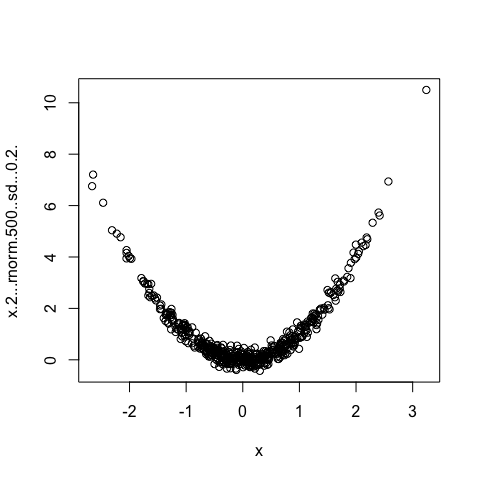
\includegraphics[width=\maxwidth]{figure/unnamed-chunk-2-1} \end{Schunk}
\caption{Verteilung von beobachteten zunehmenden Durchmesserzuwächsen (graue Balken). Wir nehmen an (in diesem Fall wissen wir es), dass diese Werte von wahren Verteilungen stammen (Population oder datengenerierender Prozess) die hier in einer rot-gestrichelten Linie angedeutet werden. Wenn wir nun mehr Daten aufzeichnen würden, würden sich die grauen Balken der wahren Verteilung immer mehr annähern.}
\label{fig: data distribution}
\end{center}
\end{figure}


Wie kann man nun die Eigenschaften der beobachteten Stichprobe zusammenfassen? Ein paar grundlegende Eigenschaften wären beispielsweise das Minimum und das Maximum, der Mittelwert, oder der Modalwert (Maximum der Verteilung). Daneben gibt es zwei weitere Kennzahlen, die von großer Wichtigkeit sind: Momente und Quantile.

Der Begriff "Moment" mag vielleicht nicht jedem geläufig sein, vermutlich haben Sie aber schon das erste und zweite Moment einer Verteilung berechnet, denn diese sind ebenfalls unter den Bezeichnungen Mittelwert und Standardabweichung bekannt. Allgemein wird das n-te Moment $\mu_n$ einer Verteilung $f(x)$ um einen Wert c definiert als 

\begin{equation}
\mu_n(c) = \int_{-\infty}^{\infty} f(x) (x - c)^n dx
\end{equation}

oder, für eine endliche Anzahl an Beobachtungen 

\begin{equation}
\mu_n(c) = \frac{1}{N}\sum_{i=1}^N (x_i - c)^n
\end{equation}

Das erste Moment mit $c=0$, ist der Mittelwert. Für die folgenden höheren Momente ist es üblich die zentralen Momente zu betrachten, die man durch das Setzen von c auf den Mittelwert erhält, da ihre Werte einfacher als Indikatoren für die Verteilungsform zu interpretieren sind.\footnote{Um die Varianz abzuschätzen, ersetzt man oft den Term 1/N durch den Bias-korrigierten Term 1/(N-1).} Die drei höheren zentralen Momente werden Varianz (n=2, identisch mit dem Quadrat der Standardabweichung, Messgröße der Streuung), Schiefe (n=3, Messgröße für die Asymmetrie in der Verteilung) und Wölbung (n=4) genannt. 

Eine zweite zentrale Kennzahl sind die Quantile. Für jede kontinuierliche Verteilung können wir die Frage stellen: Wo ist der Wert, ab dem der Messwert von einer Hälfte der beobachten Daten kleiner ist? Dieser Punkt wird als Medianwert, oder auch als 0.5-Quantil bezeichnet. Allgemeiner kann man sagen, dass die 0.x Quantile der Wert ist, an dem der Anteil 0.x des Datensatzes kleiner ist. Die 0.25 und 0.75 Quantile werden auch als 1. und 3. Quartil bezeichnet. 

\subsection{Kennzahlen der Abhängigkeit mehrerer metrischer Variablen - Korrelation}

Korrelation ist eine Kennzahl die die Abhängigkeit zweier metrischer Variablen misst. Es gibt mehrere unterschiedlich definierte Korrelationskoeffizienten. Die zwei wichtigsten sind:

\paragraph{Lineare Korrelationskoeffizienten:} Lineare Korrelationskoeffizienten messen die lineare Abhängigkeit zwischen zwei Variablen. Der wichtigste Vertreter ist der "Pearson'schen Korrelationskoeffizienten". Wegen seiner schnellen Berechnung und leichten Interpretation ist dieser Wert die Grundeinstellung in den meisten Statistikprogrammen. Man sollte bei der Interpretation beachten, dass der Koeffizient angibt, wie gut die Punkte auf einer geraden Linie liegen. Eine nichtlineare Abhängigkeit wird nicht als perfekt korreliert betrachtet, punktsymmetrische Abhängigkeiten haben grundsätzlich Korrelation Null (Fig.~\ref{fig: correlation}).

\paragraph{Rangkorrelationskoeffizienten:} Rangkorrelationskoeffizienten, wie zum Beispiel der "Spearman'sche Rangkorrelationskoeffizient" und der "Kendall Tau Rangkorrelationskoeffizient" ermitteln, wie genau die Variablen gemeinsam tendenziell steigen oder fallen, ohne hierbei das Ausmaß oder die Linearität ihrer Steigung zu beachten. Diese werden bevorzugt, wenn man von nicht-linearen Korrelationen ausgeht. 

\paragraph{Starke Korrelation != bedeutender Einfluss:} Siehe auch Fig.~\ref{fig: correlation}; ist ein oft falsch verstandener Zustand der Korrelation und Abhängigkeit - ein hoher Korrelationskoeffizient bedeutet nicht, dass eine Variable eine starke Reaktion auf eine andere bewirkt. Um eine hohe Korrelation zu erreichen braucht es nur eine geringe Streuung um die Korrelationslinie (siehe mittlere Reihe - die Auswirkung ist anders, aber die Korrelation bleibt gleich). 

% note about higher-dim correlation

\begin{figure}[htbp]
\begin{center}
\begin{Schunk}

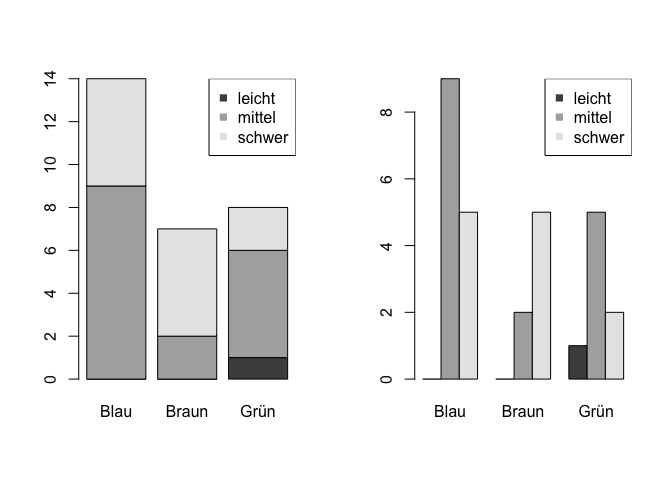
\includegraphics[width=\maxwidth]{figure/unnamed-chunk-3-1} \end{Schunk}
\caption{Beispiele einer möglichen Korrelation mit dem Pearson'schen Korrelationskoeffizienten. Beachte, dass viele Datensätze, die eine klare Abhängigkeit zwischen Variablen aufweisen, einen Pearson'schen Korrelationskoeffizienten von 0 aufweisen, da die Abhängigkeit nicht linear ist.}
\label{fig: correlation}
\end{center}
\end{figure}

\subsection{Verteilung und Abhängigkeit nichtmetrischer Variablen - Häufigkeit- und Kontingenztabellen}

Zu guter Letzt gibt es noch die klassischen Häufigkeits- und Kreuztabellen.

Eine normale Häufigkeitstabelle beschreibt die Verteilung einer nominalen oder ordinalen Variable. Eine solche Tabelle zählt einfach, wie oft verschiedene Merkmale (rot, grün, blau) in einem Datensatz vorkommen. 

Eine Kontingenztabelle (auch: Kontingenztafel oder Kreuztabelle) beschreibt, wie häufig Kombinationen von Merkmalen zweier oder mehr Variablen auftreten. Wenn man z.B. einen Datensatz mit der Variable Farbe (rot, grün, blau) und Preis (hoch, niedrig) hat, zählt die Kontingenztabelle wie oft jede Kombination (z.B. rot, hoher Preis) auftritt. 

Als\marginnote{Dieser Datensatz von Berkeley ist ein berühmtes Beispiel für das Simpson-Paradoxon. Weitere Informationen über dieses wichtige Phänomen im Abschnitt~\ref{ch: design of experiments}, Versuchsplanung.} Beispiel hier eine Kontingenztabelle eines berühmten Datensatzes aus R über die Zulassung von Hochschulbewerber in Berkeley, mit den Variablen Zulassung und Geschlecht. 

\begin{Schunk}
\begin{Sinput}
UCBAdmissions[,,1]
\end{Sinput}
\begin{Soutput}
          Gender
Admit      Male Female
  Admitted  512     89
  Rejected  313     19
\end{Soutput}
\end{Schunk}


\vspace{1cm}
\begin{fullwidth}
\begin{mdframed}[backgroundcolor=black!10,rightline=false,leftline=false]
    
\textbf{Anwendung in R:} 

Für die vielseitigen Berechnungsmöglichkeiten der deskriptiven Statistik in R, siehe \href{http://www.uni-kiel.de/psychologie/rexrepos/rerDescriptive.html}{hier}

\end{mdframed}
\end{fullwidth} 


\section{Visualisierung}

\marginnote{Gib ?anscombe in R ein, um den Code zu sehen, der diese Plots ausgibt und um die statistischen Eigenschaften des Datensatzes zu berechnen.}

Kennzahlen sind sehr nützlich, können aber auch zu Fehlinterpretationen führen. Ein bekanntes Beispiel dafür ist das Anscombe Quartett, ein hypothetischer Datensatz aus vier Stichproben, die identisch bzgl. üblicher Kennzahlen wie z.B. Mittelwert, Varianz, Korrelation, Regressionslinie, etc. sind, aber sehr unterschiedliche Verteilungen aufweisen \citep{Anscombe-Graphsinstatistical-1973}. Das Beispiel zeigt, dass die Berechnung von einfachen Kennzahlen kein vollständiger Ersatz für die graphische Darstellung der Daten darstellt.


\begin{figure}[htbp]
\begin{center}
\begin{Schunk}

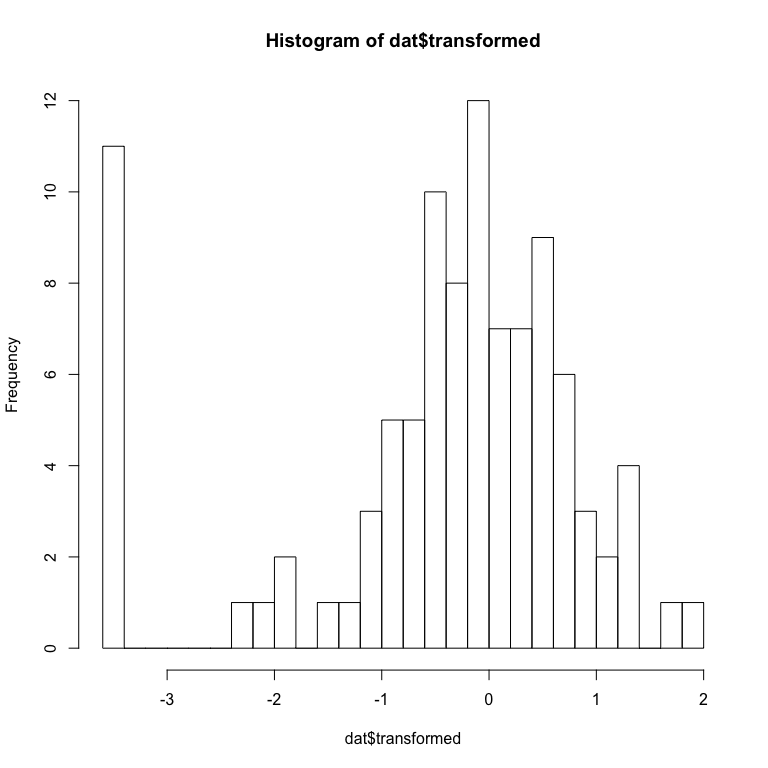
\includegraphics[width=\maxwidth]{figure/unnamed-chunk-5-1} \end{Schunk}
\caption{Anscombe's Quartet, ein hypothetischer Datensatz aus vier Variablen die identisch bzgl. üblicher Kennzahlen wie z.B. Mittelwert, Varianz, Korrelation, Regressionslinie, etc. sind, aber sehr unterschiedliche Verteilungen aufweisen.}
\label{fig: Anscombes Quartet}
\end{center}
\end{figure}

\subsection{Grundsätze der Visualisierung}

Ein Grundsatz\marginnote{Beispiele für missverständliche Abbildungen siehe \href{https://en.wikipedia.org/wiki/Misleading_graph}{hier}} von Abbildungen und Darstellungen ist, die Daten so einsehbar und wahr wie möglich darzustellen. Der Leser sollte einen bestmöglichen überblick in kürzester Zeit über die Daten erhalten. Zusätzlich sollten die Abbildungen natürlich auch anschaulich sein. Vorab ein paar generelle Tipps, die vielleicht helfen könnten:

\begin{itemize}
\item Einfach ist besser als kompliziert
\item Vermeide übertriebene Farben. Abbildungen sollten wenn möglich auch in schwarz-weiß leserlich sein (benutze einen Farbgradienten, der gleichzeitig ein Intensitätsgradient ist; benutze zusätzlich zu Farben auch gestrichelte Linien). Wenn dein Graph auf Farben basiert, achte darauf welche zu verwenden, die auch Menschen mit einer Rot-Grün-Schwäche erkennen können.
\item Ehrlichkeit: vermeide Verzerrungen. Benutze quadratische Formen, außer es gibt besondere Gründe. Achsen sollten bei 0 beginnen, außer es gibt gute Gründe, die dagegen sprechen. Verwende die gleiche Skala bei der Darstellung mehrerer Abbildungen, wenn es keine Gründe gibt, die dagegen sprechen. 
\item Manipuliere deine Abbildungen nicht!
\item Ausgabe in einem Vektor-Format (pdf, eps, svg)
\end{itemize}

\begin{figure}[htbp]
\begin{center}

\setkeys{Gin}{width=\textwidth}
\begin{Schunk}

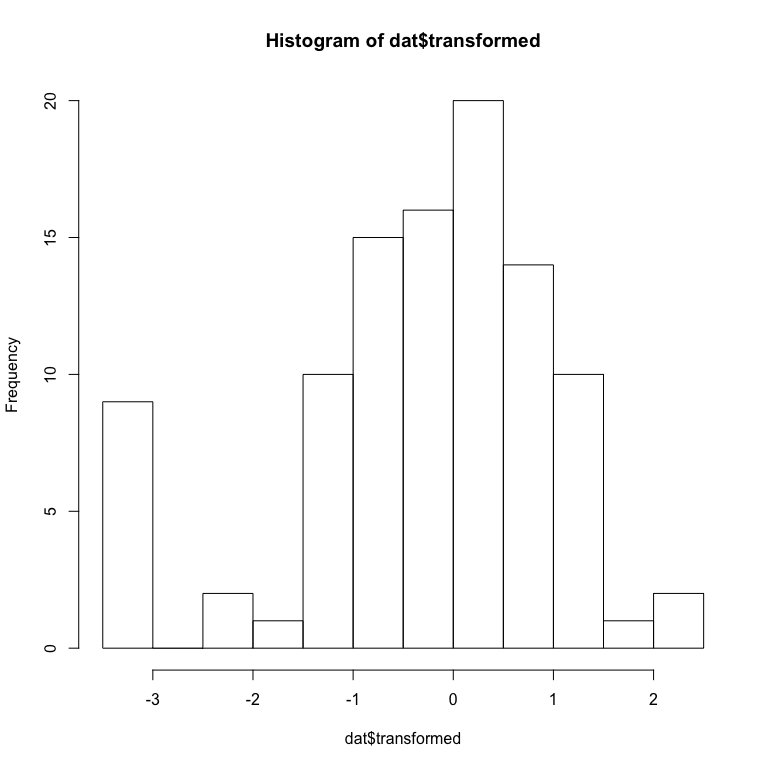
\includegraphics[width=\maxwidth]{figure/unnamed-chunk-6-1} \end{Schunk}
\caption{Vier typische Plot-Typen, von oben links nach unten rechts: a) Liniendiagramm, repräsentiert Messungen einer metrischen Variablen; b) Streudiagramm, repräsentiert eine Beziehung zwischen zweier metrischen Variablen; c) Balkendiagramm, repräsentiert Häufigkeiten Messungen in diskreten Gruppen / Variablen; d) Boxplot, repräsentiert metrische Messungen in diskreten Gruppen.}
\label{fig: exaple plots}
\end{center}
\end{figure}


\subsection{Wissenschaftliche Abbildungen}

Es gibt eine große, fast unendliche Bandbreite an verschiedenen visuellen Darstellungen von Datensätzen. Im Folgenden werden nun vier häufig verwendete Graph-Typen gezeigt. 

\paragraph{Liniendiagramme:} Liniendiagramme werden benutzt, um geordnete metrische Messwerte darzustellen. Typische Beispiele hierfür wären Zeitreihen oder mathematische Funktionen. Beispiel siehe Fig.~\ref{fig: exaple plots} a.

\paragraph{Streudiagramme:} Streudiagramme veranschaulichen zwei metrische Variablen, die paarweise gemessen wurden. Ein typisches Beispiel hierfür wäre das wiederholte Messen von verschiedenen Variablen mit der Absicht herauszufinden, ob diese korrelieren. Beispiel siehe Fig.~\ref{fig: exaple plots} b.

\paragraph{Balkendiagramme:} Balkendiagramme beinhalten Informationen (e.g. Häufigkeit oder Kennzahlen) über diskrete Gruppen. Beispiel siehe Fig.~\ref{fig: exaple plots} c.

\paragraph{Boxplots:} Boxplots benutzt man häufig bei der Verteilung einer metrischen Variable über mehrere diskrete Gruppen. Klassischerweise bestehen sie aus einer Box, 'Whiskers' (Linien) und gegebenfalls Punktewerte um die 'Whiskers'. Deren Bedeutung ist von der benutzten Software abhängig, mit der man die Plots gestaltet hat. Normalerweise bedeckt die Box die in der Mitte liegenden 50\%, mit dem angedeuteten zentralen Medianwert. Die Linien sollen zur Abschätzung der Daten-Bandbreite dienen, Ausreißer ausgenommen. Natürlich liegt es im Auge des Betrachters, was als Ausreißer angesehen wird und was nicht. Die exakte Definition von Whiskers besagt, dass die weit entfernteste Beobachtung weniger oder gleich der oberen Quantile plus 1,5 der Länge des Interquartilabstands ist. Beispiel siehe Fig.~\ref{fig: exaple plots} d.

\vspace{1cm}
\begin{fullwidth}
\begin{mdframed}[backgroundcolor=black!10,rightline=false,leftline=false]
    
\textbf{Anwendung in R:} 

Es gibt viele gute Einleitungen in Graphiken mit R, sodass diese Details hier nicht weiter aufgeführt werden. Zu Beginn empfehle ich diese  \href{https://github.com/florianhartig/ResearchSkills/tree/master/Labs/Statistics/Practicals/GraphicsInR}{übungen zum graphischen Gestalten mit R}. Diese sind begleitend zu diesem Skript, oder auch zu

\begin{itemize*}
  \item \href{http://www.statmethods.net/graphs/index.html}{QuickR}
  \item \href{http://shinyapps.org/apps/RGraphCompendium/index.php}{RGraphCompendium}
  \item \href{http://www.uni-kiel.de/psychologie/rexrepos/rerDiagrams.html}{rexrepos}
\end{itemize*}

\end{mdframed}
\end{fullwidth} 


\chapter{Schließende Statistik}\label{ch: inductive statistics}

\marginnote{Schließende Statistik ist das Ziehen von Schlüssen aus Beobachtungen durch statistische Methoden} 

Die deskriptive Statistik beschreibt unsere Daten, kann uns aber nicht sagen, ob Abhängigkeiten in den Daten systematisch oder zufällig sind. Genau dies ist das Ziel der schließenden Statistik. Ein Beispiel wäre eine klinische Studie, in der es 2 Gruppen gab, die eine (Behandlung) die ein Medikament erhalten hat, und die andere (Kontrolle) die einen Placebo erhalten hat.\marginnote{In der Statistik spricht man von "Kontrolle" wenn man Beobachtungen von Versuchseinheiten hat, an denen keine experimentelle Manipulation vorgenommen wurde. Wenn man etwas manipuliert (z.B. Medikament, Düngerzugabe, etc.) so spricht man von einer "Behandlung"} Die Ergebnisse sind dass in der Behandlungsgruppe 15/30 Patienten, und in der Kontrollgruppe 10/30 Patienten geheilt wurden. Dies können wir jetzt erst mal deskriptiv darstellen, aber die Frage an die schließende Statistik wäre: können wir davon ausgehen dass es einen Effekt der Behandlung gibt, und wenn ja, wie groß ist er wahrscheinlich?


\section{Datenerzeugendes Modell}

\marginnote{Schließende Statistik ist nicht immer, aber meist mit dem Prinzip des datengenerierenden Modells verknüpft}

Eine zentrale Idee von vielen Methoden der schließenden Statistik ist das Prinzip des datengenerierenden Modells. Das datengenerierendes Modell spezifiziert Annahmen darüber, wie die Daten entstehen (z.B. normalverteilter Fehler, lineare Abhängigkeit von einem Prädiktor). Auf diesen Annahmen aufbauend kann man dann Wahrscheinlichkeiten für die unbekannten Größen (z.B. Unterschiede zwischen Behandlungsgruppe und Kontrollgruppe) berechnen (schließen).

\begin{figure}[htbp]
\begin{center}
\begin{Schunk}

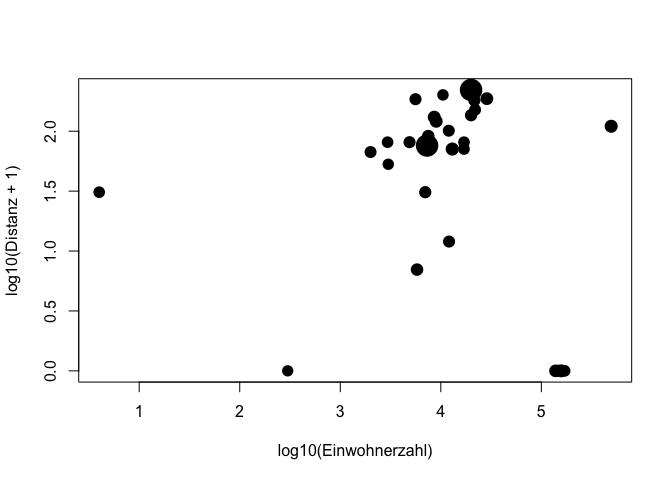
\includegraphics[width=\maxwidth]{figure/unnamed-chunk-7-1} \end{Schunk}

\caption{Beispiel: Wachstumsmessungen unter Kontrolle und zwei verschiedenen Behandlungen. Beachte die Interpretation eines Boxplots - die dickere Linie in der Mitte der Box ist der Medianwert. Die Box bedeckt das zentrale 0.5 Quantil der Verteilung}\label{fig: plant growth music}
\end{center}
\end{figure}

Ein Beispiel hierfür ist Fig.~\ref{fig: plant growth music}. Es scheint Unterschiede zwischen Kontrolle und Behandlung zu geben, jedoch gibt es auch zufällige Variation innerhalb der einzelnen Behandlungsguppen (durchschnittlich haben wir hier sieben Beobachtungen pro Behandlung). Somit könnten die Unterschiede im Mittel auch durch Zufall entstanden sein.

Wenn wir genaue Aussagen über die Wahrscheinlichkeit eines Unterschieds zwischen den zwei behandelten und der Kontrollgruppe treffen möchten, müssen wir ein Modell erstellen, welches den Zufall in den Daten beschreibt. Der übliche Ansatz ist das parametrische statistische Modell. Für die Daten könnte man z.B. annehmen, dass es eine durchschnittliche Wachstumsrate für jede Behandlungsart gibt, und das Wachstum jeder individuellen Pflanze normalverteilt um diesem Mittelwert streut. Die Parameter dieses Modells sind a) die durchschnittlichen Wachstumsraten und b) die Varianz der Normalverteilung. Diese Parameter kann man dann mit den Methoden der schließenden Statistik schätzen oder testen. 

Eine andere Möglichkeit datengenerierende Modelle zu erstellen sind nicht-parametrische Methoden.\marginnote{Die nicht-parametrische Statistik versucht Vermutungen über datengenerierende Prozesse zu vermeiden. Normalerweise entsteht der datengenerierende Prozess durch das Imitieren der eigentlichen Daten, z.B. durch das erneute Prüfen von Methoden.} Nicht-parametrische Methoden umgehen die Notwendigkeit Modellannahmen zu erstellen z.B. über Resamplingmethoden, in denen wiederholt Teile aus dem beobachteten Datensatz gezogen werden um so "künstlich" neue Daten zu generieren. Für Pflanzenwachstumsbeobachtungen unter drei verschiedenen Bedingungen (Behandlung) könnte man z.B. ein nichtparametrisches Modell für die Annahmen dass es keine Unterschiede in dem Wachstum gibt dadurch erstellen, dass man alle Beobachtungen ungeachtet der Behandlung in einen Topf wirft, sie dann zufällig den drei Gruppen zuweist, und ausrechnet wir groß die Unterschiede zwischen den Gruppen sind. Wenn wir dies nun oft wiederholen (z.B. 1000 mal) kann man einen guten Eindruck davon bekommen, wie wahrscheinlich es ist die beobachteten Unterschiede zu erhalten, wenn die Behandlungen keinen Effekt hätten.

Nicht-parametrische Methoden sind inzwischen ein wichtiger Bestandteil der modernen Statistik.\marginnote{Parametrische Methoden haben normalerweise eine höhere "Teststärke" (das Konzept wird gleich erklärt, aber grob heißt das dass sie eher einen Effekt finden wenn er da ist). Allerdings basieren alle Ergebnisse der parameterischen Statistik auf der Richtigkeit des parametrischen Modells. Wie man die Modellannahmen überprüft kann werden wir später in diesem Kapitel behandeln.} Ihr Vorteil liegt darin dass sie weniger Annahmen über die Daten treffen. Andererseits sind parametrische Methoden meist wesentlich schneller zu berechnen, und, falls ihre Annahmen korrekt sind, mit der selben Menge an Daten sensitiver (höhere Teststärke, siehe Kap.~\ref{ch: p-werte}), wodurch sie ehereinen vorhandenen Effekt erkennen. Deshalb sind die parametrische Methoden immer noch die Grundlage der meisten statistischen Analysen.

Ob parametrisch oder nicht-parametrisch, am Ende erhalten wir ein Modell dass es uns ermöglicht eine Aussage zu machen über die Wahrscheinlichkeit der Beobachtungen $D_{obs}$

\begin{equation}
p(D_{obs} | M, \Theta)
\end{equation}

gegeben unsere Modellannahmen $M$ und potentiell Parameter $\Theta$


\section{Inferentielle Outputs}

Auf diesem Modell basierend (parametrisch oder nicht-parametrisch) können wir nun verschiedene schließenden Methoden anwenden, um Schlüsse über unsere Daten zu ziehen (in unserem Beispiel: Um entscheiden zu können, ob die Behandlung einen Unterschied macht, oder nicht). In der "normalen" Statistik sind hier vor allem zwei Methoden zu nennen, die fast universell auf jedes Problem angewandt werden: p-Werte und Maximum-Likelihood-Schätzer. Außerdem wird ein weiteres drittes Verfahren momentan immer beliebter - die Posterior Wahrscheinlichkeit, die in der Bayes'schen Statistik berechnet wird. Auf diese werde ich am Ende dieses Abschnittes noch kurz eingehen.

\begin{figure}[htb]
\begin{center}
\includegraphics[width = 8cm]{InferenceDE}
\caption{Aus dem datengenerierenden Modell (parametrisch oder nicht-parametrisch) können die drei "Produkte" der schließenden Statistik gewonnen werden: a) der p-Wert, b) der Maximum-Likelihood Schätzer, und c) die Bayes'sche Posterior.}
\label{fig: InferenceMethods}
\end{center}
\end{figure}


\subsection{Hypothesentests und p-Werte}\label{ch: p-werte}

Der p-Wert ist die am häufigsten benutzte, aber leider auch am schwierigsten zu interpretierende Methode. Die Verwendung des p-Wertes basiert auf dem Ansatz des Hypothesentests (englisch: null hypothesis significance testing, NHST). Die Idee ist Folgende: wenn wir Beobachtungsdaten und ein statistisches Modell haben, können wir dieses statistische Modell benutzen, um zu testen ob die Daten zu einer festen, vorgegebenen Hypothese passen. Für das Beispiel der Pflanzen könnte unsere Hypothese so lauten: "Die Behandlung hat keinen Einfluss auf Pflanzen; alle beobachteten Unterschiede basieren auf zufälligen Abweichungen zwischen den Individuen." Dieses Szenario wird als Nullhypothese bezeichnet. \marginnote{Eine Nullhypothese $H_0$ ist ein vorgegebenes Szenario, das Vorhersagen über erwartete Wahrscheinlichkeiten von verschiedenen Beobachtungen macht.} In der Praxis wird typischerweise wird als Nullhypothese ein Szenario von "keinem" Einfluss gewählt, so dass man dann zeigen kann das es einen Einfluss gibt. Technisch könnte man aber genauso die Vermutung "Behandlung 2 verdoppelt die Wachstumsrate der Pflanzen" als Nullhypothese setzen. Es liegt im Ermessen des Analytikers, bzw. an der Fragestellung, was als Nullhypothese betrachtet werden soll. Dies ist auch der Grund für die große Auswahlmöglichkeit an verfügbaren Tests. Wir werden noch einige davon im folgenden Kapitel über wichtige Hypothesentests kennen lernen.

Nachdem\marginnote{Die Teststatstik ist eine deskriptive Statistik die die beobachteten Daten und H0 vergleicht.} wir uns für eine Nullhypothese entschieden haben, wollen wir nun feststellen ob die Daten zu der Nullhypothese passen. Die Frage ist natürlich: wie definiert man denn "passen"? Die Strategie der Hypothesentests ist sich zuerst eine Teststatistik zu definieren. Die Teststatistik ist irgendeine deskriptive Statistik die den Datensatz beschreibt (einfachstes Beispiel: der Mittelwert). Im Prinzip steht es jedem frei seine eigene Teststatistik zu wählen, aber es gibt natürlich Teststatistiken die sinnvoller sind als andere. Die Nullhypothese und die Teststatistik zusammen definieren einen Hypothesentest. 

Mit dem Hypothesentest gewappnet können wir jetzt die beobachteten Daten mit H0 vergleichen. Hierzu definieren wir den p-Wert \marginnote{Der p-Wert ist die Wahrscheinlichkeit der beobachteten Daten oder extremer, gegeben H0.} 

\begin{equation}
p := p(d >= D_{obs} | H_0)
\end{equation}

als die Wahrscheinlichkeit die beobachteten Daten oder extremer (gemessen an der Teststatsitik) zu bekommen wenn H0 wahr ist (siehe Abb.~\ref{fig: teststatistik}).


\begin{figure}[htb]
\begin{center}
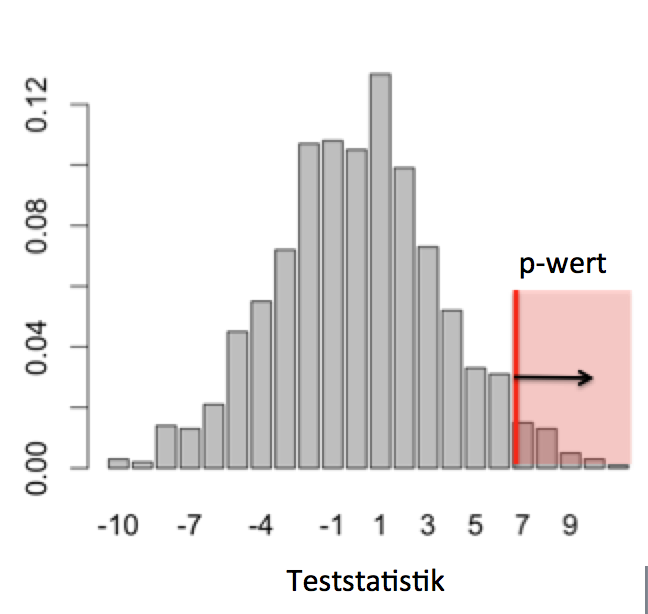
\includegraphics[width = 6cm]{Teststatistik}
\caption{Eine Visualisierung des p-Werts und der Teststatistik. Für H0 erwarten wir eine gewisse Verteilung der Teststatistik. Die beobachteten Date haben den Wert $D_obs$ der Teststatistik (rote Linie). Der p-Wert (hier ein rechsseitiger Test) ist die Wahrscheinlichkeit eine größere Teststatistik zu bekommen als der Wert für $D_obs$.}
\label{fig: teststatistik}
\end{center}
\end{figure}

Ein kleiner p-Wert zeigt also an, dass die Wahrscheinlichkeit die beobachteten Daten zu bekommen für H0 sehr klein ist. Jetzt kommt ein Trick der erst mit der weiteren Erklärung richtig sinnvoll wird: Wenn der p-Wert unter eine gewisse Schwelle sinkt (das sog. Signifikanzlevel $\alpha$), so sagt man die "Nullhypothese wird abgelehnt", "es gibt signifikante Evidenz gegen die Nullhypothese", oder einfach: "der Test / Effekt ist siginfikant". Der Wert von $\alpha$ ist eine Übereinkunft, in der Ökologie üblicherweise 0.05, sodass ein p-Wert kleiner als 0.05 ein Abweisen der Nullhypothese veranlässt. \marginnote{Wenn p<0.05, haben wir signifikante Beweise für ein Abweisen der Nullhypothese.} 

Warum diese Definition Sinn macht sieht man wenn man sich überlegt was passiert wenn man diese Regel anwendet. Zuerst: wie oft wird denn ein Ergebnis signifikant wenn H0 wahr ist? Wenn man scharf auf die Definition schaut, sieht man: genau $\alpha$. 	Man weiß also dass, wenn H0 wahr ist, man genau $\alpha$ signifikante Ergebnisse bekommt. Man nennt diese falschen Positiven den Typ I Fehler. \textbf{Der Typ I Fehler ist also immer $\alpha$}. 

Die andere Möglichkeit einen falschen Schluss zu ziehen ist, dass der Test nicht signifikant wird, obwohl H0 falsch ist. Dieses nennt man falsche Negative, oder Typ II Fehler. Den umgekehrten Wert, 1-TypII, also die Wahrscheinlichkeit Signifikanz zu bekommen wenn H0 nicht wahr ist, nennt man die Teststärke. Der Typ II Fehler ist im Allgemeinen nicht bekannt, kann aber berechnet werden wenn man den datengenerierenden Prozess und $\alpha$ kennt. Typischerweise nimmt der Fehler ab mit größerer Effektstärke, mehr Daten, größerem $\alpha$, und weniger Stochastizität (Rauschen). Ein Überblick über die Fehler beiden Fehler gibt Fig.~\ref{fig: Error Types}

\begin{figure}[htb]
\begin{center}
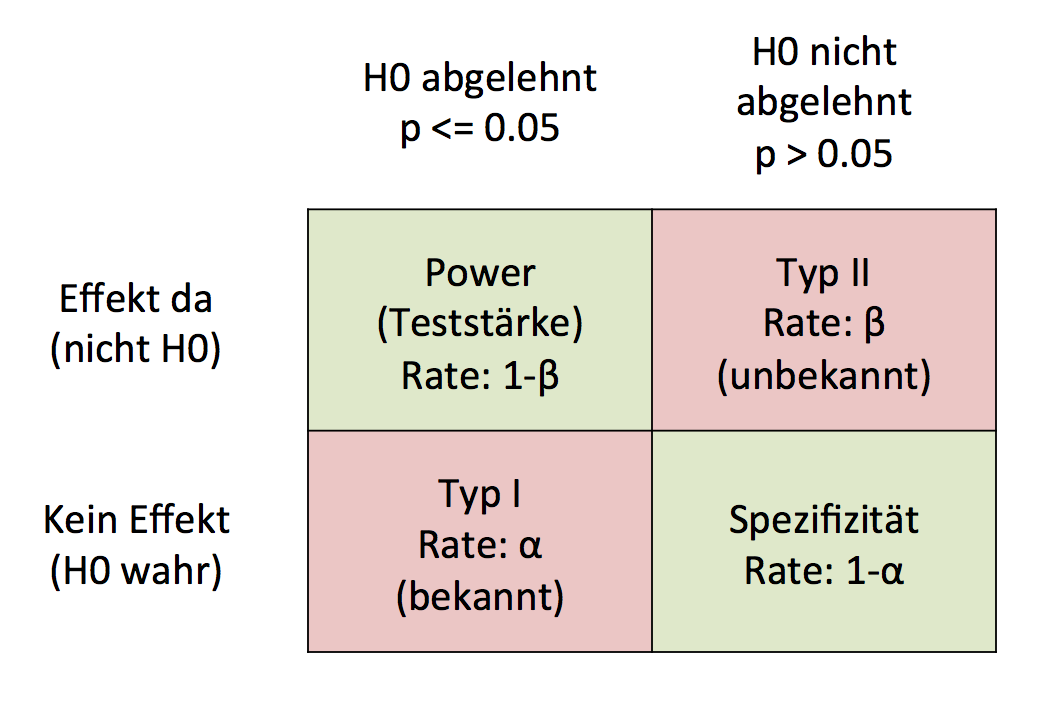
\includegraphics[width = 9cm]{ErrorTypes}
\caption{Visualisierung des TypI/II Fehlers und der Teststärke (Power).}
\label{fig: Error Types}
\end{center}
\end{figure}

Ein Problem der Hypothesentests und der p-Werte ist die notorische Fehlinterpretation der Ergebnisse. Der p-Wert ist NICHT die Wahrscheinlichkeit, dass die Nullhypothese wahr, oder die Alternativhypothese falsch ist \citep[siehe][]{Cohen-earthisround-1994}. Noch garantiert der kontrollierte Typ I Fehler, dass ein signifikantes Ergebnis mit einer festen Wahrscheinlichkeit richtig ist. 

Die Wahrscheinlichkeit, dass ein signifikantes Ergebnis falsch ist, wird durch die False Discovery Rate (FDR) beschrieben. Hierzu überlegt man sich folgendes: ein signifikantes Ergebnis kann durch 2 Wege entstehen: entweder man macht einen Typ I Fehler (Wahrscheinlichkeit $\alpha$ mal Wahrscheinlichkeit dass H0 wahr ist), oder man bekommt ein echtes positives Ergebnis (Wahrscheinlichkeit $1-\beta$ (Teststärke) mal Wahrscheinlichkeit dass H0 wahr ist). Dies ist in Fig~\ref{fig: FDR} dargestellt. Also kann man die FDR ausrechnen
\begin{equation}
FDR := \frac{p(H0) \cdot \alpha}{ p(H0) \cdot \alpha + p(!H0) \cdot (1-\beta)}
\end{equation}

Solange man neben $\alpha$ auch die Teststärke und $p(H0)$ kennt. Beachte: aus der Formel sieht man dass die FDR typischerweise wesentlich höher ist als 5\%. Man sollte also signifikante Ergebnisse mit der entsprechenden Vorsicht genießen. Die FDR ist höher a) je kleiner die Teststärke ist, und b) je wahrscheinlicher H0 ist. 

% Zitat hier


\begin{figure}[htb]
\begin{center}
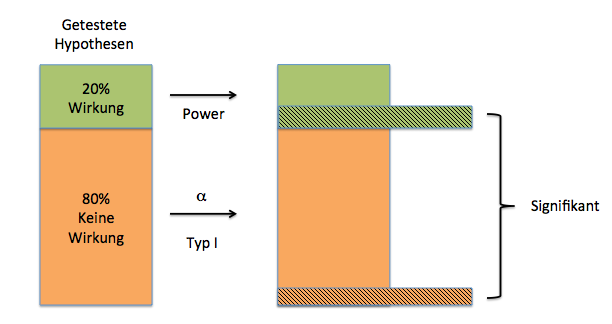
\includegraphics[width = 11cm]{FDR}
\caption{Visualisierung der False Discovery Rate (FDR)}
\label{fig: FDR}
\end{center}
\end{figure}


\subsection{Maximum-Likelihood-Schätzwert}

Das zweite zentrale Verfahren der schließenden Statistik ist die Methode der Maximum Likelihood Schätzer (maximum-likelihood estimate, MLE). Für diese Methode betrachtet man die Wahrscheinlichkeit der beobachteten Daten als Funktion der Modellparameter $\theta$ 

\begin{equation}\label{eq: likelihood}
L(\theta) := p(D_{obs} | M(\theta))
\end{equation}

Der Maximum-Likelihood-Schätzer\marginnote{Merke: der Maximum Likelihood Schätzer ist der Parametersatz, für den die Daten am wahrscheinlichsten sind, nicht jedoch der wahrscheinlichste Parametersatz!} ist die Parameterkombination, für welche die Wahrscheinlichkeit in eq.~\ref{eq: likelihood}. 

Der Maximum-Likelihood-Schätzung (MLE) ist eine "Punktschätzer" (engl: point estimate), weil nur ein Parameterwert berechnet wird.\marginnote{Eine Punktschätzung ist vergleichbar mit einer einzelnen besten Schätzung.} Ein einzelner Wert ist aber oft nicht besonders nützlich, weil man nicht weiß, wie unsicher er ist.\marginnote{Das Konfidenzintervall beschreibt die Unsicherheit um die Punktschätzung} Deswegen wird der MLE normalerweise mit einem Konfidenzintervall angegeben. Ein korrekt definiertes 95\% Konfidenzintervall überdeckt bei wiederholten Experimenten den wahren Parameter in 95\% aller Fälle. Salopp gesagt ist das Konfidenzintervall ist der ungefähre Bereich, in dem wir den korrekten Parameter erwarten. 

\vspace{1cm}
\begin{fullwidth}
\begin{mdframed}[backgroundcolor=black!10,rightline=false,leftline=false]
    
\textbf{Übungsfragen MLE:} 
\textbf{4.1} Wie ist die Likelihood der beobachteten Daten D für ein gegebenes Modell M mit Parameter x definiert?
\textbf{4.2} In einem Experiment wurde der Effekt von Stickstoff auf das Wachstum von Pflanzen getestet - die Likelihood ist maximal für eine Verdoppelung des Wachstums. Die Autoren schreiben: “Die Wahrscheinlichkeit die beobachteten Daten zu erhalten ist maximal wenn man annimmt dass Stickstoff das Wachstum von den beobachteten Pflanzen verdoppelt” - ist diese Aussage korrekt?
\textbf{4.3} Weiter unten schreiben die Autoren: “Der wahrscheinlichste Wert für den Effekt von Stickstoff ist 2 (Verdoppelung)” - ist diese Aussage korrekt?

\end{mdframed}
\end{fullwidth}

\subsection{Bayes Verfahren}

Unsere\marginnote{Die Bayes'sche Statistik berechnen eine dritte Größe, die Posterior Wahrscheinlichkeit.} Übersicht der schließenden Methoden wäre nicht komplett ohne eine dritte Methode zu erwähnen, die Bayes'sche Statistik. In der Bayes'schen Statistik wird eine dritte Größe berechnet, die Posterior Wahrscheinlichkeit. Diese ist ähnlich, jedoch nicht identisch zu MLE. Die Bayes'sche Statistik wird bei komplizierteren Modellen sehr wichtig, hier wollen wir aber nicht weiter darauf eingehen. Bei Bedarf und Interesse hilf \citet{Gelman-BayesianDataAnalysis-2003} und diese \href{http://florianhartig.github.io/LearningBayes/}{Webseite}.

\subsection{Verschiedene Methoden != verschiedene Modelle}

Wir kennen nun die drei Methoden der schließenden Statistik (Hypothesentests, Maximum-Likelihood, und Bayes), und wissen dass diese drei verschiedene Größen liefern: p-Wert, MLE und die Posterior. 

\marginnote{ANOVA , t-Tests und lineare Regression sind nur unterschiedliche Begutachtungen des selben Modells} 
Ein häufiges Missverständnis besteht darin, die Auswertungsmethode mit dem Modell zu verwechseln. Ein Beispiel hierfür sind die nun folgenden Methoden ANOVA, t-Tests und die lineare Regression. Alle basieren auf ein und dem selben datengenerierenden Modell. Nur legen ANOVA und t-Tests verschiedenste Nullhypothesen fest, und die lineare Regression sucht nach dem MLE. 

\section{Wichtige Hypothesentests}

Nachdem jetzt die grundlegenden statistischen Datenausgaben besprochen wurden, gehen wir nun in die Praxis über, um die zwei wohl häufigsten Hypothesentests kennenzulernen - den t-Test und ANOVA. Wie bereits erwähnt, basieren beide auf dem selben datengenerierenden Prozess, legen jedoch geringfügig unterschiedliche Nullhypothesen fest.

\subsection{t-Test}

Der t-Test testet auf Unterschiede in den Mittelwerten zweier normalverteilter Stichproben; oder im Falle einer einzigen Stichprobe auf einen Unterschied des Mittelwerts der Stichprobe zu 0. Die Nullhypothese ist, dass es keine Unterschiede zwischen den Mittelwerten der zwei normalverteilten Gruppen gibt, bzw., wenn wir nur eine Gruppe betrachten, dass der Stichprobenmittelwert 0 ist. 

In dem meisten Programmen gibt es eine Reihe von Optionen für den t-Test. Die wichtigsten sind a) ob die beiden Gruppen die gleiche Varianz haben, und b) Ob die Stichproben in Paaren gesammelt wurden, d.h. ob jeweils eine Beobachtung aus beiden Gruppen irgendwie verbunden sind (z.B. vorher / nachher). Diese Einstellungen können einen großen Effekt haben, es ist daher wichtig die Hilfe richtig zu lesen. 

Hier ein Beispiel für den t-Test in R, mit klassischen Daten von \citet{Student-probableerrormean-1908}. Die Daten zeigen die Wirkung von zwei Schlafmitteln (gesteigerte Anzahl an Schlafstunden verglichen mit der Kontrolle) an 10 Patienten. 



\begin{figure}[htbp]
\begin{center}
\begin{Schunk}

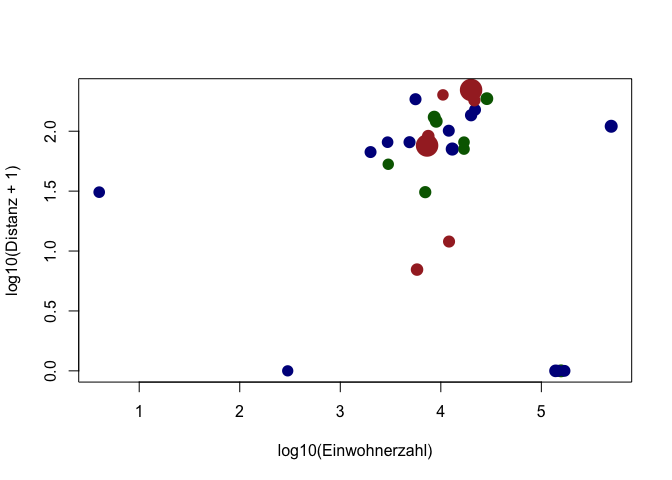
\includegraphics[width=\maxwidth]{figure/unnamed-chunk-8-1} \end{Schunk}
\caption{Daten von \citet{Student-probableerrormean-1908}}
\label{fig: Student Sleep Data}
\end{center}
\end{figure}

\begin{Schunk}
\begin{Sinput}
## Traditional interface
with(sleep, t.test(sleep$extra[sleep$group == 1], extra[group == 2]))
\end{Sinput}
\end{Schunk}

\begin{Schunk}
\begin{Sinput}
## Formula interface
t.test(extra ~ group, data = sleep)
\end{Sinput}
\begin{Soutput}

	Welch Two Sample t-test

data:  extra by group
t = -1.8608, df = 17.776, p-value = 0.07939
alternative hypothesis: true difference in means is not equal to 0
95 percent confidence interval:
 -3.3654832  0.2054832
sample estimates:
mean in group 1 mean in group 2 
           0.75            2.33 
\end{Soutput}
\end{Schunk}

Zu beachten ist, dass die Funktion einen p-Wert (H0 = kein Unterschied), aber auch einen MLE mit Konfidenzinterval ausgibt. Dies geht also über den klassischen T-Test hinaus. Vermutlich nahmen die Programmierer an, dass man zusätzlich den besten Schätzwert für die Mittelwertsunterschiede haben möchte.

Hier ein Vorschlag für die verbale Kommunikation der Ergebnisse: wenn p>0.05: Unterschiede zwischen den Gruppen waren nicht signifikant. Wenn p<0.05: Wir erhielten einen Unterschied von X +- Konfidenzintervall zwischen den Gruppen (p-Wert für die Unterschiede eines T-Tests mit X). 


\subsection{Varianzanalyse (ANOVA)}

Die Definition der ANOVA (analysis of variance) oder Varianzanalyse ist nicht ganz eindeutig. Die klassische ANOVA macht grundsätzlich die gleichen Annahmen wie ein t-Test (normalverteilte Resonanz), jedoch für mehr als zwei Gruppen. Genauer gesagt testet sie, ob die gemessene abhängige Variable von einer oder mehrerer kategorialer Variablen beeinflusst wird, und wie sich der Einfluss auf die verschiedenen Variablen aufteilt. Es können auch Interaktionen beachtet werden. Eine Interaktion\marginnote{Interaktion: eine Variable verändert den Effekt der anderen Variablen. Beispiel: die Variable Geschlecht könnte eine Auswirkung darauf haben wie gut ein Medikament wirkt. Es besteht also potentielle eine Interaktion zwischen Geschlecht und Behandlung.} zwischen zwei erklärenden Variablen bedeutet, dass sich der Wert der einen auf den Effekt der anderen Variable auswirkt. 

Wir werden später lernen, dass die normale lineare Regression (die die gleichen Annahmen macht wie t-Tests und klassische ANOVA) auf andere Verteilungsannahmen erweitert werden kann. Hierdurch gelangt man zu den sogenannten generalisierten linearen Modellen. Das Prinzip der ANOVA lässt sich auch auf diese Modelle anwenden, und dies wird dann oft auch einfach als ANOVA bezeichnen. Deshalb Vorsicht: normalerweise heißt ANOVA = Normalverteilung, aber oft wird der Begriff auch wesentlich breiter verwendet.

Hier ist ein einfaches Beispiel mit einer Standard-ANOVA (normalverteilte Fehler), in der getestet werden soll, ob Gewicht (von Hühnern) von ihrer Ernährung abhängt, wobei 'Ernährung' ein Faktor mit vier Möglichkeiten ist:

\begin{Schunk}
\begin{Sinput}
aovresult <- aov(weight~Diet, ChickWeight)
summary(aovresult)
\end{Sinput}
\begin{Soutput}
             Df  Sum Sq Mean Sq F value   Pr(>F)    
Diet          3  155863   51954   10.81 6.43e-07 ***
Residuals   574 2758693    4806                     
---
Signif. codes:  0 '***' 0.001 '**' 0.01 '*' 0.05 '.' 0.1 ' ' 1
\end{Soutput}
\end{Schunk}

Wir erhalten einen p-Wert von 6.43e-07, welcher mit unseren normalen Signifikanzniveau $\alpha=0.05$ höchst signifikant ist. Somit können wir die Nullhypothese (H0: die Ernährung hat keinen Einfluss auf die abhängige Variable "Gewicht") ablehnen. 

Ein Problem der ANOVA ist, dass wir keine Parameterschätzwerte erhalten und deshalb keine Aussagen darüber machen können, welche Ernährung nun am besten ist, oder welche sich von welcher unterscheidet. Man hat jetzt 2 Möglichkeiten

\begin{itemize}
\item Entweder wendet man den sogenannten Post-Hoc-Test an, welcher auf Unterschiede der Paaren von Ernährungsweisen testet (Bsp. mit einem t-Test).
\item Oder man wechselt zu einer Regression, die im folgenden Kapitel genauer beschrieben wird.
\end{itemize}

\paragraph{Multiples Testen}\marginnote{Beim Anwenden multipler Tests auf die selben Daten benötigt man eine Korrektur des p-Werts für multiples Testen.} Typischerweise macht man nicht einen, sondern mehrere Post-Hoc-Test. Dies kann zum Problem werden - der Grundgedanke des p-Werts ist dass der Typ I Fehler fest ist, aber dass man nur einen Test macht. Wenn man nun mehrere Tests macht, aber gerne immer noch eine 5\% Typ I Fehlerrate bei einem $\alpha$ Level von 0.05 hätte, muss man für multiples Testen korrigieren.  

\subsection{Weitere wichtige Tests}

Es gibt natürlich wesentlich mehr Hypothesentests als wir hier durchgenommen haben. Eine Liste mit wichtigen Tests gibt es beispielsweise auf \href{http://en.wikipedia.org/wiki/Category:Statistical_tests}{Wikipedia}. Niemand kann alle Tests auswendig kennen. Der Trick ist sich genau zu überlegen welche Nullhypothese man testen will, und sich dann den entsprechenden Test zu suchen. Eine hervorragende Resource ist die Liste von gebräuchlichen Tests auf  \href{http://www.ats.ucla.edu/stat/mult_pkg/whatstat/}{hier}, zusammen mit der praktischen Anwendung in R auf \href{http://www.ats.ucla.edu/stat/r/whatstat/whatstat.htm}{hier}.

\vspace{1cm}
\begin{fullwidth}
\begin{mdframed}[backgroundcolor=black!10,rightline=false,leftline=false]
    
\textbf{Übungsfragen Hypothesentests:} 
\textbf{4.4} Definieren Sie den p-Wert.
\textbf{4.5} Wie ist in der vorherigen Definition “extremer” (also >=) definiert?
\textbf{4.6} Stellen Sie sich vor Sie leben in Venedig, und es gibt 3 Taxibootfirmen. Sie wollen wissen ob es Unterschiede in der Beförderungsgeschwindigkeit gibt und machen deshalb 300 Fahrten mit jeder Firma und stoppen die Zeit. Was wäre eine geignete Nullhypothese H0, um auf einen Unterschied zu testen?
\textbf{4.7} Bonusfrage: Nennen Sie eine der vielen möglichen sinnvollen Teststatistiken
\textbf{4.8} In der Physik gibt es das sogenannte Standardmodell, dass die Eigenschaften und Interaktionen der Material beschreibt. In den letzten 20 Jahren wurde das Standardmodell immer und immer wieder getestet, so “erfolgreich” dass die Physiker schon ein bisschen deprimiert sind weil Sie nichts neues entdecken. Was ist die Nullhypothese die bei diesen Tests angewandt wird?
\textbf{4.9} Sie lesen einen Artikel über ein medizinisches Experiment. Getestet wurde ein Medikament gegen eine Kontrolle, und der p-Wert ist 0.03. Die Studie schreibt: “Die Wahrscheinlichkeit dass das Medikament nicht wirkt ist 3\%” - stimmen Sie zu?
\textbf{4.10} Schreiben Sie eine korrekte Interpretation des obigen Ergebnis auf.
\textbf{4.11} Definierent Sie den Typ I Fehler (falschen positive).
\textbf{4.12} Wie viel Typ I Fehler erwarten Sie bei einen Signifikanzlevel von 7\%?
\textbf{4.13} Definieren Sie den Typ II Fehler (falsche negative).
\textbf{4.14} Wie viel Typ II Fehler erwarten Sie bei einen Signifikanzlevel von 7\%?
\textbf{4.15} Nennen Sie 2 Faktoren die Typ II Fehler beeinflussen, und die Richtung des Einflusses (negativ = Typ II nimmt ab wenn Faktor hoch geht).
\textbf{4.16} Definieren Sie die Teststärke / Power.
\textbf{4.17} Sie testen 100 Gene auf eine Assoziation mit Krebs. Bei 5 Genen zeigt der Test Signifikanz an. Wie bewerten Sie dieses Ergebnis?
\textbf{4.18} Sie bekommen von einer allwissenden Macht die Zusatzinformation dass Sie in dem oben genannten Test eine Teststärke von 99\% hatte. Sind Sie nun zuversichtlicher dass Sie einen Effekt gefunden haben?
\textbf{4.19} Definieren Sie die False Discovery Rate (FDR).
\textbf{4.20} Wovon hängt die FDR ab?
\textbf{4.21}  In einer Reihe von Experimenten testen Sie Medikamente auf eine Wirkung. Ihre Power ist 100\%. Sie schätzen dass jedes 20. Medikament das Sie testen eine Wirkung haben solte. Wie ist ihre FDR bei einem Signifikanzlevel von 5\%? Es reicht wenn Sie den Rechenweg aufschreiben, Sie müssen den Wert nicht ausrechnen.

\end{mdframed}
\end{fullwidth}



\section{Lineare Regression}

Wie zuvor schon angedeutet liegt der Regression nicht unbedingt ein anderes statistisches Modell zugrunde als den Hypothesentests. Genauer gesagt: die lineare Regression, die wir als erstes kennenlernen, macht im Prinzip die gleichen Annahmen wie t-Test und ANOVA. Der Unterschied besteht in der schließenden Methode. Während die Hypothesentests p-Werte berechnen, berechnet die Regression den Maximum-Likelihood-Schätzer für eine vom Nutzer vorgegebene potentielle Abhängigkeit zwischen der abhängigen Variable und den Prädiktoren.

Das einfachste Regressionsmodell ist die einfache lineare Regression. Das Wort "einfach" bedeutet in diesem Zusammenhang: es gibt nur einen Prädiktor. Wenn es mehr als einen Prädiktor gibt, spricht man von einer "multiplen" lineare Regression. Bei der einfachen linearen Regression lautet die Annahme, dass wir eine abhängige Variable haben, die von einem Prädiktor wie folgt abhängt:

\begin{equation} \label{eq: linear regression}
y \sim a \cdot x + b + \epsilon 
\end{equation}

Hier ist y die abhängige Variable, x der Prädiktor, a, b sind die zu schätzenden Parameter die die Abhängigkeit zwischen y und x beschreiben, und  $\epsilon$ steht für eine normalverteilte Zufallsvariable. In R führt man eine solche Regression durch den folgenden Befehl aus

\begin{Schunk}
\begin{Sinput}
fit = lm(airquality$Temp~airquality$Ozone)
\end{Sinput}
\end{Schunk}

Die Funktion sucht den MLE, also die Parameterwerte (Achsenabschnit und Steigung für Temperatur), für die die Wahrscheinlichkeit der beobachteten Daten maximal wird. Das Ergebnis können wir uns mit der summary Funktion anschauen

\begin{Schunk}
\begin{Sinput}
summary(fit)
\end{Sinput}
\begin{Soutput}

Call:
lm(formula = airquality$Temp ~ airquality$Ozone)

Residuals:
    Min      1Q  Median      3Q     Max 
-22.147  -4.858   1.828   4.342  12.328 

Coefficients:
                 Estimate Std. Error t value Pr(>|t|)    
(Intercept)      69.41072    1.02971   67.41   <2e-16 ***
airquality$Ozone  0.20081    0.01928   10.42   <2e-16 ***
---
Signif. codes:  0 '***' 0.001 '**' 0.01 '*' 0.05 '.' 0.1 ' ' 1

Residual standard error: 6.819 on 114 degrees of freedom
  (37 observations deleted due to missingness)
Multiple R-squared:  0.4877,	Adjusted R-squared:  0.4832 
F-statistic: 108.5 on 1 and 114 DF,  p-value: < 2.2e-16
\end{Soutput}
\end{Schunk}

Diese MLEs werden unter "Estimate" ausgegeben. Dies zeigt uns, wie sehr der Prädiktor, in diesem Fall Ozon, die abhängige Variable, hier Temperatur, beeinflusst: Für jede Einheit Ozon mehr steigt die Temperatur um 0.201 Einheiten, mit einem Standardfehler (Konfidenzintervall) von 0.019. 

Zusätzlich wird die Unsicherheit (Konfidenzinterval) für jeden Schätzer ausgegeben (Std. Error, 1.96*Std. Error entspricht dem 95\% Konfidenzinterval), und ein p-Wert für die Nullhypothese dass der Parameter 0 ist.  %Dieser p-Wert basiert auf einem bestimmten Typ von T-Test, wobei das vollständige Modell gegen ein Modell mit auf 0 gesetzten Parametern getestet wird. Zusätzlich gibt es noch einen weiteren p-Wert, welcher auf einer anderen Testgröße am Ende der Regressionsausgabe beruht. Dieser testet die Nullhypothese mit allen Parametern gleich 0.

Die Regressionstabelle sagt uns also: 

\begin{itemize}
\item Was der "Best-Guess" für die Abhängigkeit ist (Estimate)
\item Wie unsicher man ist (Std. Error)
\item Ob es signifikante Evidenz gibt gegen H0: die Abhängigkeit ist 0 
\end{itemize}

Fig~\ref{fig: lineareRegression} zeigt das Ergebnis auch noch mal visuell. Bei der Interpretation dieser Zahlen ist zu beachten: Korrelation ist nicht Kausalität. Wir haben hier die Temperatur als abhängige Variable und Ozon als Prädiktor benutzt haben, aber dies bedeutet nicht, dass Ozon ursächlich die Temperatur beeinflusst. \marginnote{Korrelation ist nicht Kausalität.}Tatsächlich ist es wohl eher anders herum: wenn wir mehr Sonne haben, wird es wärmer und wir haben tendenziell mehr Ozon. Was die Regression sagt ist: wenn unsere Ozonmessungen steigen, können wir ziemlich sicher davon ausgehen können, dass es auch gleichzeitig wärmer wird. Das bedeutet aber nicht zwingend, dass Ozon Hitze erschafft. Wie wir aus diesem Dilemma kommen besprechen wir in Kapitel~\ref{ch: design of experiments}. Für den Moment halten wir fest: Korrelation ist nicht Kausalität!


\begin{figure}[htbp]
\begin{center}
\begin{Schunk}

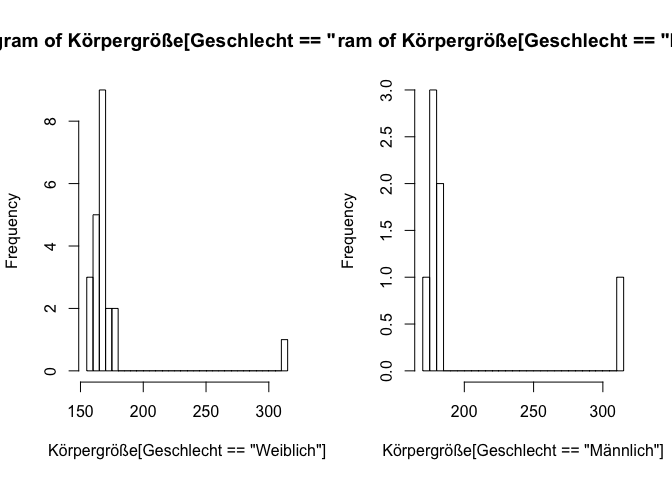
\includegraphics[width=\maxwidth]{figure/unnamed-chunk-14-1} \end{Schunk}
\caption{Temperatur aufgetragen gegen Ozon, zusammen mit der gefitteten Regressionsgraden. }
\label{fig: lineareRegression}
\end{center}
\end{figure}


%Dieser Code kann unabhängig davon verwendet werden, ob der Prädiktor metrisch oder kategorisch ist. Im Falle einer metrischen Variable entsteht eine Linie anhand der Daten. Im Falle einer kategorischen Variable mit n Stufen ist die erste Stufe als Referenz gesetzt (Schnittpunkt), und n-1 Faktoren entsprechen den folgenden Stufen, die den Unterschied zur Referenz beschreiben.

\vspace{1cm}
\begin{fullwidth}
\begin{mdframed}[backgroundcolor=black!10,rightline=false,leftline=false]
    
\textbf{Spezifizierung von verschiedenen Modellannahmen in R:} 

Die abhängige Variable y hängt linear von Variable a (metrisch oder kategorisch) ab

\begin{Schunk}
\begin{Sinput}
fit = lm(y~a)
summary(fit)
\end{Sinput}
\end{Schunk}

Die abhängige Variable y hängt linear von zwei Variablen a und b (metrisch oder kategorisch) ab, aber der Wert beider Variablen beeinflusst nicht den Effekt, welcher die andere Variable auf die abhängige Variable hat (keine Interaktion)

\begin{Schunk}
\begin{Sinput}
fit = lm(y~a+b)
summary(fit)
\end{Sinput}
\end{Schunk}

Die abhängige Variable y hängt linear von zwei Variablen a und b (metrisch oder kategorisch) ab, aber der Wert der einen Variable beeinflusst nicht den Effekt der anderen Variable auf die abhängige Variable (Interaktion)

\begin{Schunk}
\begin{Sinput}
fit = lm(y~a*b)
summary(fit)
\end{Sinput}
\end{Schunk}

Die abhängige Variable y ist von einer Variablen a (metrisch oder kategorisch) wie in $a + a^2$ abhängig

\begin{Schunk}
\begin{Sinput}
fit = lm(y~a + I(a^2))
summary(fit)
\end{Sinput}
\end{Schunk}

Bemerkung: so ein quadratische Zusammenhang wird immer noch als lineare Regression bezeichnet. Das Wort "linear" steht dafür dass die Parameter lineare in die Regressionsgleichung eingehen, und nicht für einen linearen Zusammenhang. Bemerkung 2: Die Schreibweise I() kennzeichnet eine darauf folgende mathematische Formel. 

\end{mdframed}
\end{fullwidth}



\subsection{Überprüfen der Modellannahmen}

Technisch kann man fast jeden Datensatz mit einer linearen Regression schätzen, ohne dass die Software zusammenbricht. Dies heißt allerdings nicht dass man das tun sollte. In der Statistik gilt immer: die Ergebnisse basieren auf den Annahmen der Methode. Wenn Sie diese Annahmen verletzten, kann alles passieren, im Zweifel sind die Ergebnisse wahrscheinlich falsch. Es ist also immer wichtig die Annahmen der Regression zu überprüfen.

Also was genau waren die Annahmen einer linearen Regression? Richtig, Normalverteilung! Ein häufiger Fehler ist an diesem Punkt den Prädiktor oder die abhängige Variable auf Normalverteilung zu überprüfen. Das bring gar nichts. Schauen Sie auf die Formel ~\ref{eq: linear regression}. Wenn man die Formel umstellt, sieht man dass der folgende Ausdruck

\begin{equation} \label{eq: residuals}
res_i = y_i - (a \cdot x_i + b ) \sim \epsilon 
\end{equation}

nämlich der Unterschied zwischen beobachtetem Wert und den Modellvorhersagen, normalverteilt sein sollte. Die Werte $res_i$, also der Unterschied zwischen Modellerwartung und Daten, heißen die Residuen. Jeder Datenpunkt hat sein Residuum. 

Also, wir müssen die Residuen überprüfen. Da man nur Residuen erhält wenn man auch ein Modell fittet, heißt das: wir können nicht a priori sagen ob man einen Datensatz mit der linearen Regression fitten darf. Wir probieren es erst mal aus, und dann schauen wir uns im Nachhinein an den Residuen an ob das OK war. Die einfachste Methode hierfür ist die Residuen gegen die erwarteten Werte zu plotten. 



\begin{figure}[htbp]
\begin{center}
\begin{Schunk}

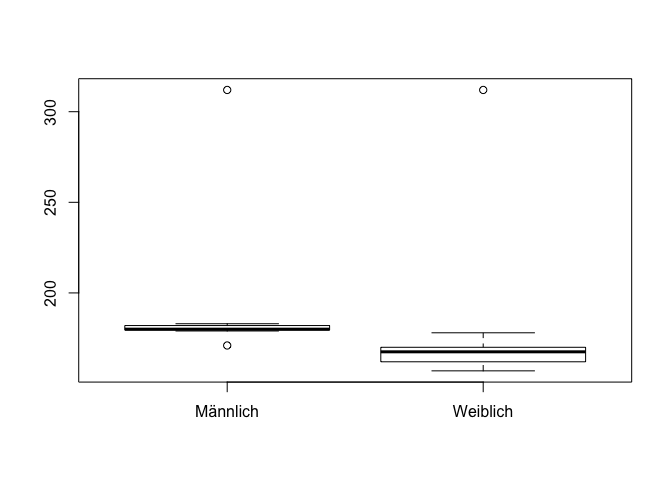
\includegraphics[width=\maxwidth]{figure/unnamed-chunk-19-1} \end{Schunk}
\caption{Eine Sammlung möglicher Muster, wenn die Residuen gegen den angepassten Wert (voreingestellt in R) oder einen Prädiktor geplottet werden.}
\label{fig: ResidualPatterns}
\end{center}
\end{figure}

In Fig.~\ref{fig: ResidualPatterns} sind typische Probleme dargestellt die in einen solchen Residuenplot auftreten können. Die wichtigsten sind:

\begin{itemize}
  \item Heteroskedastizität (Varianzinhomogenität): hier ändert sich die Breite der Streuung, eine Verletzung der Regressionsannahme dass die Normalverteilung eine feste Varianz hat. 
  \item Muster in den Residuen: wenn an ein Muster in den Residuen sieht heißt dass typischerweise, dass man die falsche Funktion fittet. 
  \item Verteilung nicht normal: tja, wenn sie nicht normalverteilt ist, dann ist das natürlich schlecht, denn das ist die Annahme der linearen Regression. 
\end{itemize}  

Es gibt weitere spezialisierte Plots, um mit der Diagnose dieser Probleme zu helfen. Diese erfolgen bei der Anwendung des Befehls plot(fit). Weitere Details zur Residuendiagnose siehe \href{http://www.statmethods.net/stats/rdiagnostics.html}{hier}.


\section{Generalisierte lineare Regressionsmodelle (GLM)}

Die Annahmen der linearen Regression waren, dass 1) die abhängige Variable metrisch ist (Wertebereich im Prinzip von - unendlich bis + unendlich), und 2) dass die Residuen normalverteilt sind. 

Die Idee der GLMs ist, das allgemeine Prinzip der LMs beizubehalten, den Wertebereich und die Verteilung aber zu modifizieren. Dazu geschehen zwei Dinge

\paragraph{Die Link-Funktion:} Um den Wertebereich zu modifizieren, wendet man auf die Erwartung der normalen linearen Regression eine Transformation, die sogenannte Link-Funktion, an. Wir haben gesagt, dass eine lineare Regression folgende Form annimmt

\begin{equation}
y \sim a \cdot x + b 
\end{equation}

Das heißt, je nach Werten von a, x könnte y jeden Wert einnehmen, positiv oder negativ. Ein Trick, um sicherzustellen, dass alle Vorhersagen für y positiv sind oder innerhalb eines bestimmten Bereichs liegen, ist eine Link-Funktion der Form

\begin{equation}
y \sim f^{link}(a \cdot x + b )
\end{equation}

Im Prinzip gibt es bei der Wahl kein Einschränkung, aber es gibt ein paar typische Funktione die benutzt werden, z.B. die Exponentialfunktion, die positive Ergebnisse garantiert, oder der inverse Logit, der Bereich zwischen 0 und 1 garantiert.

\paragraph{Andere Verteilungen:} Nachdem wir den Wertebereich modifiziert haben können wir jetzt auch über andere Verteilungen nachdenken. Zwei typische Entscheidungen, die wir unten verwenden, sind die Binomial- (die Verteilung für das Münzwerfen) und die Poisson-Verteilung (eine diskrete Wahrscheinlichkeitsverteilung). Es stehen viele andere Möglichkeiten zur Verfügung. Vielleicht wird die Idee noch deutlicher, wenn wir uns in den nächsten Abschnitten zu den konkreten Beispielen bewegen.

\subsection{0/1 Daten - logistische Regression}

Die logistische Regression ist die Standardoption für binäre Daten (1/0, Anwesend / Abwesend, überlebt / tot, infiziert / nicht infiziert). Logistische Regression geht davon aus, dass die Verteilung binomial ist (Münzwurf-Modell). Um den Wertebereich der linearen Regression auf eine Skala zwischen 0 und 1 zu transformieren, verwenden wir die logistische Linkfunktion (oder inverse Logit), und danach die Binominialverteilung.

\vspace{1cm}
\begin{fullwidth}
\begin{mdframed}[backgroundcolor=black!10,rightline=false,leftline=false]
    
\textbf{Anwendung in R:} 

Hier ein Beispiel mit den Daten der Titanik-überlebenden. Beachte, dass die Logit-Link automatisch ausgewählt wird, wenn in R die Binomialverteilung verwendet wird. Bei Bedarf könnte man diese Wahl überschreiben.

\begin{Schunk}
\begin{Sinput}
library(effects)
fmt <- glm(survived ~ age + I(age^2) + I(age^3), family=binomial, data = TitanicSurvival)
summary(fmt)
\end{Sinput}
\begin{Soutput}

Call:
glm(formula = survived ~ age + I(age^2) + I(age^3), family = binomial, 
    data = TitanicSurvival)

Deviance Residuals: 
    Min       1Q   Median       3Q      Max  
-1.5062  -0.9978  -0.9695   1.3483   2.0135  

Coefficients:
              Estimate Std. Error z value Pr(>|z|)    
(Intercept)  7.855e-01  3.031e-01   2.592 0.009549 ** 
age         -1.189e-01  3.291e-02  -3.613 0.000303 ***
I(age^2)     3.414e-03  1.113e-03   3.066 0.002171 ** 
I(age^3)    -2.931e-05  1.107e-05  -2.648 0.008109 ** 
---
Signif. codes:  0 '***' 0.001 '**' 0.01 '*' 0.05 '.' 0.1 ' ' 1

(Dispersion parameter for binomial family taken to be 1)

    Null deviance: 1414.6  on 1045  degrees of freedom
Residual deviance: 1398.5  on 1042  degrees of freedom
  (263 observations deleted due to missingness)
AIC: 1406.5

Number of Fisher Scoring iterations: 4
\end{Soutput}
\end{Schunk}


\end{mdframed}
\end{fullwidth} 


\subsection{Zähldaten - Poisson-Regression}

Die Poisson-Regression ist die Standardoption für Zähldaten. Zähldaten sind immer positiv. In der Poisson-Regression wird deshalb normalerweise eine Exponentialfunktion gewählt, um alle Werte positiv zu machen. Das Inverse des Exponentials ist der Log, also nennen wir das den Log-Link. R wählt diesen Link wieder automatisch aus, wenn als Verteilung "family = poisson" angibt.

\vspace{1cm}
\begin{fullwidth}
\begin{mdframed}[backgroundcolor=black!10,rightline=false,leftline=false]
    
\textbf{Anwendung in R:} 

Als Beispiel, hier ein Test ob Vogeleltern ihren Kindern mehr Futter geben wenn sie attraktiver sind. 


\begin{Schunk}
\begin{Sinput}
schnaepper <- read.csv("schnaepper.txt", sep="")
fm <- glm(stuecke ~ attrakt, family=poisson, data = schnaepper)
summary(fm)
\end{Sinput}
\begin{Soutput}

Call:
glm(formula = stuecke ~ attrakt, family = poisson, data = schnaepper)

Deviance Residuals: 
     Min        1Q    Median        3Q       Max  
-1.55377  -0.72834   0.03699   0.59093   1.54584  

Coefficients:
            Estimate Std. Error z value Pr(>|z|)    
(Intercept)  1.47459    0.19443   7.584 3.34e-14 ***
attrakt      0.14794    0.05437   2.721  0.00651 ** 
---
Signif. codes:  0 '***' 0.001 '**' 0.01 '*' 0.05 '.' 0.1 ' ' 1

(Dispersion parameter for poisson family taken to be 1)

    Null deviance: 25.829  on 24  degrees of freedom
Residual deviance: 18.320  on 23  degrees of freedom
AIC: 115.42

Number of Fisher Scoring iterations: 4
\end{Soutput}
\end{Schunk}

\end{mdframed}
\end{fullwidth} 


%\subsection{Residuen-überprüfungen in allgemeinen linearen Regressionsmodellen}

%Residuen in generalisierten linearen Modellen sind per Definition nicht normalverteilt, deshalb bringt es wenig die 

%in allgemeinen linearen Regressionsmodellen sollten nicht normalverteilt sein, deswegen verwendet man keine Standard-Kontrollen für Normalität wie normale Quantile-Quantile-Plots, um auf die Angemessenheit der Residuen zu überprüfen. Für nicht zu komplizierte Modelle gibt es eine Möglichkeit dieses Problem zu umgehen, indem man die sogenannten Pearsons-Residuen verwendet, die die beobachteten Unterschiede zwischen Modell und Daten durch die erwartete Varianz des Modells normiert \footnote{In R kann man die Option Pearson in vielen Funktionen angeben, einschließlich der Residual()-Funktion, die man auf ein angepasstes Objekt anwenden kann}

%Ein Standardproblem in Poisson oder binomialen allgemeinen linearen Regressionsmodellen ist, dass die Varianz der Poisson- und Binomialverteilung nicht eingestellt werden kann, sondern durch den Mittelwert festgelegt wird. Dies ist ein Problem, das im normalen linearen Modell nicht auftritt, da hier der zufällige Teil durch eine Normalverteilung modelliert wird, die einen Parameter für die Varianz aufweist. Ein Problem, das sehr häufig in Poisson oder binomialen allgemeinen linearen Regressionsmodellen auftritt, ist eine überdispersion, d.h. dass die Residuen mehr Varianz, als unter dem angepassten Modell erwartet, zeigen. \marginnote{Man kann auf überdispersion prüfen, indem man die angepasste Abweichung betrachtet oder einen überdispersionstest anwendet} Der einfachste Weg, um dies zu korrigieren, ist die Verwendung der Quasi-Poisson- und Quasibinomialmodelle, die in der allgemeinen linearen Regressionsmodell-Funktion verfügbar sind. Diese Modelle bringen einen zusätzlichen Parameter ein, der die Varianz des Poisson- und des binomialen allgemeinen linearen Regressionsmodells abwandelt.

\vspace{1cm}
\begin{fullwidth}
\begin{mdframed}[backgroundcolor=black!10,rightline=false,leftline=false]
    
\textbf{Übungsfragen Regression:} 
\textbf{4.22} Was sind die Annahmen der linearen Regression?
\textbf{4.23} Wie werden die Parameter in der linearen Regression bestimmt?
\textbf{4.24} Welche H0 steckt hinter den p-Werten der Parameter der linearen Regression?

\end{mdframed}
\end{fullwidth}


\chapter{Prädiktive Statistik und Maschinelles Lernen}\label{ch: Prädiktive Statistik}

Prädiktive Statistik (auch: maschinelles Lernen) ist ein dritter Bereich der Statistik, der in den letzten Jahren zunehmend an Bedeutung gewonnen hat. Das grundlegende Ziel dieser Methoden besteht darin, gute Vorhersagen aus einem komplexen Datensatz zu erzeugen. Dabei verwenden sie typischerweise relativ komplizierte, nicht-parametrische Verfahren, die Vorhersagen ermöglichen, aber keine Berechnung klassischer Größen der schließenden Statistik, wie z.B. der p-Wert oder MLE. 

Die vielleicht bekannteste Methode des maschinellen Lernens ist der sogenannte Random Forest Algorithmus. Genau zu erklären wie dieses Algorithmus funktioniert würde hier zu weit führen, aber um eine grobe Idee zu geben: die Idee ist die Daten durch sogenannten Entscheidungsbäume zu beschreiben. Die Entscheidungsbäume sagen: Daten mit Eigenschaft A führen zu Ergebnis X, und Eigenschaft B führt zu Y. Eine Strategie für Vorhersagen wäre jetzt einen sehr detaillierten Entscheidungsbaum zu bauen. Genau das mach der Random Forest nicht. Statt dessen baut er viele einfache (= schlechte) Entscheidungsbäume und kombiniert diese dann. Erstaunlicherweise führt die Kombination von vielen schlechten Modellen oft zu einer besseren Vorhersage als die eines guten Modells. Hier ein Beispiel des Algorithmus, in dem wir die Menge an Ozon in der Luft aus verschiedenen anderen Wetterparametern voraussagen 

Mit der klassischen linearen Regression können wir ungefähr 60\% der Varianz in Ozon erklären

\begin{Schunk}
\begin{Sinput}
ozone.lm <- lm(Ozone ~ ., data=airquality, na.action=na.omit)
summary(ozone.lm)
\end{Sinput}
\begin{Soutput}

Call:
lm(formula = Ozone ~ ., data = airquality, na.action = na.omit)

Residuals:
    Min      1Q  Median      3Q     Max 
-37.014 -12.284  -3.302   8.454  95.348 

Coefficients:
             Estimate Std. Error t value Pr(>|t|)    
(Intercept) -64.11632   23.48249  -2.730  0.00742 ** 
Solar.R       0.05027    0.02342   2.147  0.03411 *  
Wind         -3.31844    0.64451  -5.149 1.23e-06 ***
Temp          1.89579    0.27389   6.922 3.66e-10 ***
Month        -3.03996    1.51346  -2.009  0.04714 *  
Day           0.27388    0.22967   1.192  0.23576    
---
Signif. codes:  0 '***' 0.001 '**' 0.01 '*' 0.05 '.' 0.1 ' ' 1

Residual standard error: 20.86 on 105 degrees of freedom
  (42 observations deleted due to missingness)
Multiple R-squared:  0.6249,	Adjusted R-squared:  0.6071 
F-statistic: 34.99 on 5 and 105 DF,  p-value: < 2.2e-16
\end{Soutput}
\end{Schunk}

Random Forest schafft es auf 70\%. Wir haben hier keine Vorhersagen auf neue Daten getestet, aber typischerweise fällt der Unterschied zwischen lm und rf in diesem Fall noch deutlicher aus. 

\begin{Schunk}
\begin{Sinput}
library(randomForest)
ozone.rf <- randomForest(Ozone ~ ., data=airquality, mtry=3,
                         importance=TRUE, na.action=na.omit)
print(ozone.rf)
\end{Sinput}
\begin{Soutput}

Call:
 randomForest(formula = Ozone ~ ., data = airquality, mtry = 3,      importance = TRUE, na.action = na.omit) 
               Type of random forest: regression
                     Number of trees: 500
No. of variables tried at each split: 3

          Mean of squared residuals: 276.6565
                    % Var explained: 74.79
\end{Soutput}
\end{Schunk}

Der Random Forest liefert keine p-Werte o.ä., aber man kann sich wenigsten die Wichtigkeit der verschiedenen Variablen anzeigen lassen, wobei sich hier Wichtigkeit auf die Wichtigkeit für die Vorhersage bezieht, eine kausale Annahme wird hier nicht gemacht. 


\begin{figure}[htbp]
\begin{center}
\begin{Schunk}

\includegraphics[width=\maxwidth]{figure/unnamed-chunk-24-1} \end{Schunk}
\caption{Wichtigkeit der Variablen im geschätzten Random Forest Modell.}
\label{fig: Variable Importance Random Forest}
\end{center}
\end{figure}


Das Verhältnis zwischen den Anhängern der klassischen schließenden Statistik und den maschinellen Lernen ist seit langem von Spannungen geprägt. Klassische Statistiker bemängeln dass das maschinelle Lernen die Idee des "Lernens von Daten" im Sinne des Vergleichens von Hypothesen und Daten zugunsten einfacher Prognosen aufgegeben hat. Ein Anhänger des maschinellen Lernens würde darauf antworten, dass es bei vielen angewandten Problemen nicht um das Testen von kausalen Zusammenhängen, sondern nur um das Erkennen von Pattern geht. Das Ziel ist es, einen Algorithmus zu erstellen, der in der Lage ist bei einem komplexen Datensatz korrekt vorherzusagen. \footnote{Typische maschinelle Lernanwendungen beinhalten die Vorhersage der Interessen der Kunden in Web-Shops, die Korrelation komplexer Satellitendaten mit Bodensignalen oder Sprach/Gesichtserkennung.} Der Erfolg ist auf der Seite des maschinellen Lernens: Experten in diesem Feld sind derzeit bei Technologieunternehmen wie Google, Facebook, etc. heiß begehrt, und der Markt scheint immer weiter zu wachsen. Der Unterschied zwischen der schließenden und der prädiktiven Statistik sowie die Spannung zwischen diesen Bereichen ist Inhalt des äußerst empfehlenswerten Artikels "Statistical Modeling: The Two Cultures" von \citet{Breiman-StatisticalModelingTwo-2001}, dem Erfinder des Random Forest Algorithms. Hier ein Auszug aus diesem Text:

\begin{quote}
There are two cultures in the use of statistical modeling to reach conclusions from data. One assumes that the data are generated by given stochastic data model. The other uses algorithmic models and treats the data mechanism as unknown. The statistical community has been committed to the almost exclusive use of data models. This commitment has led to irrelevant theory, questionable conclusions, and has kept statisticians from working on a large range of interesting current problems. Algorithmic modeling, both in theory and practice, has developed rapidly in fields outside statistics. It can be used both on large complex data sets and as a more accurate and informative alternative to data modeling on smaller data sets. If our goal as a field is to use data to solve problems, then we need to move away from exclusive dependence on data models and adopt a more diverse set of tools.
\end{quote}

Eine abschließende Bemerkung: Aufgrund der großen und wachsenden Bedeutung der prädiktiven Methoden in der modernen Statistik habe ich dieses kurze Kapitel in diesen Einführungstext aufgenommen. Natürlich gibt es wesentlich mehr zu diesem Thema zu sagen als der Platz hier erlaubt. Um mehr über prädiktive Methoden zu lernen würde ich Ihnen die sehr lesbaren Artikel \citet{Breiman-StatisticalModelingTwo-2001, Shmueli-Toexplainor-2010} sehr ans Herz legen, außerdem das Lehrbuch von \citet{James-IntroductiontoStatistical-2013}, das ich auch am Ende dieses für die weitere Lektüre empfehle. Es ist instruktiv zu sehen wie viel Interesse diesen Methoden im Internet entgegengebracht wird, und dass viele Firmen offene Wettbewerbe in prädikativer Statistik ausschreiben um Mitarbeiter zu gewinnen (siehe, z.B. \href{kaggle.com}{https://www.kaggle.com/}). 


\chapter{Versuchsplanung}\label{ch: design of experiments}

Kommen wir zurück zum Anfangspunkt dieses Skripts: den Daten. Wenn wir selbst Daten erheben, müssen wir eine Reihe von Fragen beantworten: Welche Variablen sollten gemessen werden? Wie variieren wir Variablen, über die wir Kontrolle haben. Und wie viele Replikate brauchen wir?


\section{Auswahl der Variablen}

In der Praxis interessieren wir uns typischerweise dafür, wie eine abhängige Variable von einer Anzahl von Prädiktoren beeinflusst wird. Wenn uns diese Beziehung interessiert, müssen wir logischerweise sowohl die abhängige Variable als auch die Prädiktoren messen.\marginnote{Korrelation ist keine Kausalität.} Eine minimale Anforderung ist weiter, dass wir verschiedene Werte der Prädiktoren haben sollten (wenn sich die Prädiktoren nicht ändern können wir auch keine Abhängigkeit beweisen). Normalerweise interessiert uns aber nicht nur Korrelation, sondern wir wollen auch mit einiger Sicherheit sagen können ob diese Korrelation kausal ist. Hierzu müssen wir alternative Erklärungen ausschließen. Variablen die als alternative Erklärung in Betracht kommen werden als Störfaktoren bezeichnet.

\subsection{Was ist ein Störfaktor?}

Stellen wir uns vor wir wollen wissen ob A von B abhängt, also $A \sim B$. Was passiert, wenn es einen zweiten Prädiktor C gibt, der auch A beeinflusst, uns aber eigentlich nicht interessiert? In Englischen nennt man C "extraneous variable", im Deutschen gibt es dafür leider keine gängige Übersetzung. \marginnote{Eine "extraneous variable" ist eine Variable, die die abhängige Variable beeinflussen kann, aber für den Experimentator nicht von Interesse ist.}. Also, es gibt auch $A \sim C$, aber diese Beziehung interessiert uns nicht. Die Korrelation $A \sim C$ ist es normalerweise kein Problem, solange C mit B unkorreliert ist. Wenn man in einem solchen Fall C missachtet, passiert normalerweise kein großer Schaden (es könnte sein, dass die unerklärte Varianz des Modells etwas höher ist, dadurch p-Werte etwas beeinflusst werden).

\begin{figure}[]
\begin{center}
\includegraphics[width = 6cm]{Confounding}
\caption{Visualisierung eines Störfaktors. Eine wichtige Voraussetzung für einen Störfaktor ist, dass die Variable sowohl mit der abhängige Variable korreliert als auch mit den Prädiktorvariablen, die unsere ursprüngliche Hypothese bilden. Wenn die zweite Verbindung nicht vorhanden ist, ist die Variable nicht störend und kann ignoriert werden.}
\label{fig: Confounding}
\end{center}
\end{figure}

Die Variable C wird zu einem Problem wenn Sie auch mit B korreliert. Dann nennt man C einen Störfaktor.\marginnote{Eine Störfaktor ist eine externe Variable, die sowohl mit der abhängigen Variable, als auch mit einer primär interessanten Prädiktorvariable korreliert.} Wenn wir in diesem Fall nur $A  \sim B$ messen, erscheint in der Korrelation $A \sim B$ auch die Auswirkungen von B und C auf A. In diesem Fall kann es passieren, dass eine Korrelation zwischen $A \sim B$ erscheint, obwohl A gar nicht mit B, sondern nur mit C kausal zusammenhängt.\marginnote{Eine Scheinkorrelation ist eine Korrelation, die durch einen Störfaktor verursacht wird.} Dieses Phänomen wird als Scheinkorrelation bezeichnet. Wenn der geschätze Effekt von $A \sim B$ falsch ist weil ein Störfaktor in in der Analyse bedacht wurde, so wird dies als omitted variable bias (OVB) bezeichnet. Eine extreme Version davon ist Simpson's Paradoxon. Simpson's Paradoxon beschreibt das Phänomen, dass ein Störfaktor die Richtung der Korrelation $A \sim B$ (Vorzeichen) umdrehen kann, so dass der Anschein besteht als ob der Einfluss in B umgekehrt ist als der wahre Einfluss. 


\subsection{Was macht man mit Störfaktoren?}

Im experimentellen Design gibt es drei Optionen, um den Einfluss von Störfaktoren zu minimieren:

\begin{enumerate}
\item Kontrolle: Entweder man hält den Faktor fest, oder man variiert ihn in kontrollierter Weise (siehe unten).
\item Randomisierung: Randomisierung heißt dass der experimentelle Aufbau eine Korrelation zwischen den gewünschten erklärenden Variablen und möglichen Störfaktoren unterbindet, e.g. durch geeignete Durchmischung. 
\item Messen: Wenn Störfaktoren gemessen sind kann man sie später durch die Statistik rausrechnen. Ein Problem hier ist dass hierdurch oft die Teststärke (Power) deutlich abnimmt
\end{enumerate}

Natürlich können die drei Techniken auch kombiniert werden. 


\section{Definition und Messfehler von Variablen}

Nach der Entscheidung WAS gemessen werden soll geht es jetzt um das WIE. Ein häufiger Fehler bei diesem Schritt des experimentellen Desigs ist es die Messungen für selbstverständlich zu erachten, und sich jetzt direkt mit der Anzahl an Replikaten usw. auseinanderzusetzen. Erst sollten wir uns aber fragen:\footnote{Die Betrachtung dieser beiden Fragen wird oft als Konstruktvalidität bezeichnet.}

\begin{enumerate}  
  \item Misst mein Versuchsaufbau, was ich messen möchte
  \item Was ist der erwartete statistische (stochastische) Fehler in meinen Messungen und was ist der mögliche systematische Fehler?
\end{enumerate}

\begin{figure}[]
\begin{center}
\includegraphics[width = 10cm]{RandomizedBlockDesign}
\caption{Illustration eines randomisierten Blockdesigns, der wohl am häufigsten verwendeten Anordnung bei (Beobachtungs)-Experimente zur Randomisierung der Auswirkung unbekannter und nicht gemessener verwandter Variablen. Die Idee dieses Entwurfs ist, dass die unbekannten Variablen wahrscheinlich im Raum korrelieren. Indem wir alle experimentell verändernden Variablen zu einem Block zusammenfassen, vermeiden wir, dass sie von den unbekannten räumlichen Variablen gestört werden können.}
\label{fig: RandomizedBlockDesign}
\end{center}
\end{figure}


Der erste Punkt mag auf den ersten Blick ein wenig seltsam erscheinen. Doch in vielen Fällen der ökologischen Statistik und darüber hinaus messen wir nicht direkt die Variable an der wir interessiert sind, sondern einen Stellvertreter (Proxy). Vielleicht wollen wir die Temperatur an einer bestimmten Stelle wissen, verwenden hierzu aber die Temperatur von einer Wetterstation in 5 km Entfernung. Oder wir wollen die funktionale Vielfalt untersuchen, aber die können wir nicht direkt messe - Zugriff haben wir auf Artendiversität - ist das ein guter Proxy?

Die zweite Frage bezieht sich darauf, wie sehr sich zwei Messungen voneinander unterscheiden würden, wenn wir sie wiederholt durchführen (stochastischer Fehler) und wie viele Messungen systematisch ausfallen könnten (systematischer Fehler, oder auch Bias), z.B. weil eine Methode oder ein Instrument systematisch falsch ist oder weil der Mensch bestimmte Einflüsse zeigt.


\section{Auswahl der Werte für die unabhängigen (Prädiktor-) Variablen}

Inzwischen wissen, wir welche Prädiktoren wir messen wollen, und wie. Normalerweise haben wir Einfluss auf die Auswahl der Werte der Prädiktoren (z.B. weil wir Manipulationen an dem System vornehmen). Wir müssen uns also jetzt überlegen wie wir die Werte variieren. 

In\marginnote{Die experimentelle Einheit ist die Einheit, die einer bestimmten Variablenkombination (z.B. Behandlung oder Kontrolle) zugewiesen werden kann. Beispiel: eine einzelne Pflanze oder ein Topf.} einer experimentellen Studie haben wir in der Regel eine Versuchseinheit (experimental unit), z.B. eine Pflanze, ein Topf oder eine Versuchsfläche, und diese Einheit wird dann manipuliert. Auch Beobachtungsstudien haben Versuchseinheiten (das was man beobachtet), aber es ist meist nicht möglich, die Prädiktoren vollständig zu kontrollieren. Allerdings hat man in der Regel die Möglichkeit bestimmte Selektionen vorzunehmen. Dies ist wichtig, denn in jedem Fall benötigt man eine ausreichende Variation der Prädiktorvariablen um eine aussagekräftige statistische Analyse zu gewährleisten.

Hier sind ein paar Punkte, die bei der Planung zu beachten sind

\subsection{Kollinearität der Prädiktoren}

In Beobachtungsstudien kommt es oft vor dass 2 Prädiktoren korrelieren (Kollinearität). Wenn man an einer der beiden nicht interessiert ist, ist diese ein Störfaktor. Aber selbst wenn man an beiden interessiert ist, so ist die Statistik mit Kollinearität normalerweise problematischer zu rechnen. Bei der Versuchsplanung sollte man alles tun um die Kollinearität möglichst klein zu halten. 

\subsection{Interaktionen}

Um Interaktionen zwischen Variablen erkennen zu können, genügt es nicht, jede Variable unabhängig zu verändern, sondern es bedarf bestimmter Kombinationen. Das Schlagwort hier ist (fractional) faktorielle Designs. Google wird hier weiterhelfen.

\subsection{Nichtlineare Effekte}

Die Verbindung von zwei Punkten ist eine Linie. Wenn man herausfinden möchte, ob die abhängige Variable auf eine Variable nichtlinear ist, benötigt man daher mehr als zwei Werte für jede Variable (Faustregel >4). 


\section{Wie viele Replikate?}

Wie wir gelernt haben, ist der Typ I Fehler unabhängig von der Anzahl der Datenpunkte. Was sich ändert ist Teststärke (engl. power) = 1 - Typ II Fehler (falsche Negative), und FDR. \marginnote{Teststärke ist die Wahrscheinlichkeit, Signifikanz für einen Effekt zu finden, wenn es welche gibt}. Im Allgemeinen 

\begin{enumerate}
\item steigt die Teststärke wenn die Effekte stärker sind und die Daten mehr
\item sinkt die Teststärke wenn die Variabilität zunimmt, oder wenn man $\alpha$ erhöht
\end{enumerate}

In den meisten Fällen kann man Effektstärken, Rauschen etc. aus Erfahrung abschätzen. Dann kann man in einer Poweranalyse berechnen wir, wie viele Replikate benötigt werden, um eine bestimmte Tesstärke zu erreichen. Hier ein Beispiel in R für den t-Test, dass zeigt dass wir bei einem Gruppenunterschied von 1, Varianz 1.5 ungefähr 50 Replikate benötigen um eine Tesstärke von 0.9 zu erreichen. 

\begin{Schunk}
\begin{Sinput}
power.t.test(power = .90, delta = 1, sd = 1.5)
\end{Sinput}
\begin{Soutput}

     Two-sample t test power calculation 

              n = 48.26431
          delta = 1
             sd = 1.5
      sig.level = 0.05
          power = 0.9
    alternative = two.sided

NOTE: n is number in *each* group
\end{Soutput}
\end{Schunk}





\newpage
\begin{fullwidth}
\begin{mdframed}[backgroundcolor=black!10,rightline=false,leftline=false]
    
\textbf{Checkliste für die Versuchsplanung}

\begin{description}

\item[( )] Eindeutige, logische Frage? Schriftlich festhalten.

\item[( )] Frage auf Validität checken, siehe hier \href{http://florianhartig.github.io/ResearchSkills/}{http://florianhartig.github.io/ResearchSkills/}

\item[( )] Versuchsplan

  \begin{description}

  \item[( )] Festlegen der zu messenden Variablen. Entscheide, ob man an linearen Hauptauswirkungen oder auch an nichtlinearen Effekten oder Interaktionen interessiert ist.
  
  \item[( )] Potenzielle Störfaktoren? Entscheide, ob sie besser kontrolliert, randomisiert oder gemessen werden sollten. Sind Kandidaten sicher störend (korreliert mit abhängige Variable UND einem oder mehreren der Prädiktoren)?
  
  \item[( )] Definiere final die zu testende statistische Hypothese, einschließlich der Störfaktoren. Festhalten, z.B. in der Form $height  \sim age + soil * precipitation + precipitation^2$. 
  
  \item[( )] Wähle aus, wie die Variablen im Experiment variiert werden. Ziehe die Verwendung von Software dafür in Betracht, z.B. für faktorielle Versuchsplanungen (in Beobachtungsstudien hat man manchmal begrenzte Kontrolle, aber man kann vielleicht schätzen, welche Variablenkombinationen beobachtet werden).
  
  \item[( )] Blocking - versuche, verschiedene Behandlungen / verschiedenste Kombinationen zusammen zu gruppieren. Das Ziel ist, dass unbekannte / nicht gemessene Variablen nicht mit experimentellen Variablen korrelieren (siehe Pseudoreplikation).
  
  \item[( )] Bestimme die Anzahl der Replikate. Mache eine Vermutung für Effektgröße und Variabilität der Daten, und berechne oder errate die Anzahl der notwendigen Wiederholungen, um genügend Teststärke zu erhalten. Was genügend bedeutet, hängt vom Sachgebiet ab, aber ich würde behaupten, dass du eine hohe Chance haben möchtest, einen Effekt zu sehen, wenn einer da ist, also wäre eine Teststärke von $>80\%$ gut.
  
  \end{description}
  
\item[( )] Versuchsaufbau prüfen.
  
  \begin{description}
  
  \item[( )] Spiele den Versuchsablauf durch, entweder in Kopf, als Pilotstudie, oder am Computer. 
  
  \item[( )] Spiele die Datenanalyse durch! Komplette Auswertung

  \end{description}


\item[( )] überarbeite alles, wenn nötig

\end{description}

\end{mdframed}
\end{fullwidth}


\chapter{Wissenswertes und weiterführende Literatur}

\section{Reproduzierbarkeit und gutes wissenschaftliches Arbeiten}

Reproduzierbarkeit bedeutet, dass jeder Schritt der Analyse wiederholbar ist. Die Erfahrung zeigt, dass es nicht so trivial ist, wie man denkt, die Reproduzierbarkeit zu gewährleisten. Hier einige Hinweise, wie man Datenanalyse reproduzierbar machen kann

\begin{itemize}

\item{Sobald man Rohdaten produziert hat: speichern, Backup, und nie mehr ändern}

\item{"Cleaning", Umbenennung etc. vor der Datenanalyse wenn möglich durch ein Skript (z. B. R, Python, perl). Wenn es absolut notwendig ist mit Hand/Maus zu arbeiten (ist es fast nie), eine Kopie des Datensatzes erstellen und jede Eingabe schriftlich dokumentieren.}

\item{Verwende ein Versionskontrollsystem für den Code und notiere für jede Ausgabe die Revisionsnummer, mit der die Ausgabe erstellt wurde.}

\item{Wenn die Analyse durchgeführt wird, speichere die random-seed und die Einstellungen des Computers, um die Reproduzierbarkeit sicherzustellen. In R ist der einfachste Weg dies zu tun, die random-seed auf random.seed(123) zu setzen und die Ergebnisse von sessionInfo(), welche die Versionsnummern aller verwendeten Pakete enthält, zu speichern.}

\item{Denke darüber nach, den Code in einer Reporting-Umgebung wie z.B. Rmd oder sweave auszuführen.}


%\footnote{Siehe auch die R-Task-Ansicht über \href{https://cran.r-project.org/web/views/ReproducibleResearch.html}{reproduzierbare Forschung}

\end{itemize}

\section{Weiterführende Literatur}\label{sec: further readings}


\begin{itemize}


\item Als praktisches Lehrbuch für Anfänger empfehle ich als deutsche Option  \citet{Dormann-ParametrischeStatistik-2013} oder Dormann, C. \& Kühn, I. (2011) Angewandte Statistik fuer die biologischen Wissenschaften (kostenloses Skript \href{https://www.biom.uni-freiburg.de/mitarbeiter/dormann/resolveuid/ed4f35206584421e7406414aa2d4470a}{hier}, und \citet{Gotelli-PrimerEcologicalStatistics-2004} als englische Option. 

\item Technisch etwas anspruchsvoller (aber immer noch sehr elementar) ist \citet{James-IntroductiontoStatistical-2013}. Man kann sich das PDF kostenlos herunterladen und es gibt ein MOOC mit Vorträgen und Übungen

\item Weitere Hilfe und Hinweise kann man in der Statistik-Hilfe unserer Abteilung \href{http://biometry.github.io/APES/}{hier} finden; siehe insbesondere die Empfehlungen zu Lehrbüchern \href{http://biometry.github.io/APES/Stats/stats90-references.html}{hier}.

\end{itemize}


\bibliographystyle{chicago}
\bibliography{/Users/Florian/Home/Bibliography/Databases/flo}


\begin{appendices}

\vspace{1cm}
\begin{fullwidth}
%\begin{mdframed}

\chapter{Lösungen der Übungsfragen}

\textbf{4.1} p(D|M,x) - in Worten: die Wahrscheinlichkeits(dichte) für D, gegeben M und x.
\textbf{4.2} Ja.
\textbf{4.3} Nein. Der MLE gibt den Wert für den die Wahrscheinlichkeit der Daten maximual ist. Um die Aussage umzudrehen müssen wir Zusatzannahmen machen (alle Parameter gleich wahrscheinlich).
\textbf{4.4} p(d >= D | H0), in Worten: Wahrscheinlickhkeit die beobachteten oder extremere Daten zu bekommen wenn H0 wahr ist.
\textbf{4.5} Extremer bezieht sich auf die Teststatistik - diese ist ein Abstandsmaß dass der “Erfinder” des Testes wählt. Weil es hierfür unterschiedliche Möglichkeiten gibt gibt durchaus verschiedene Tests mit gleichen H0, aber anderen Teststatistiken.
\textbf{4.6} H0: Die durchschnittliche Zeit aller 3 Firmen ist gleich.
\textbf{4.7} Mögliche Antworten: Varian der 3 Mittelwerte, Unterschied größter / kleinster Mittelwert, Durchschnitt der Differenzen der Mittelwerte, … [alles womit man die Firmen vergleichen könnte .. natürlich könnten Sie auch Mittewert durch Median ersetzen].
\textbf{4.8} H0 = das Standardmodell.
Anmerkung: ich wollte Ihnen mit diesem Beispiel zeigen dass es 2 Möglichkeiten gibt Nullhypothesen aufzustellen: Wenn wir einen Effekt bestätigen wollen, stellen wir die umgekehrte Nullhypothese auf, also dass es keinen Effekt gibt (das ist der Normalfall in der Analyse von biologischen Daten). Der Hintergrund hier ist dass wir einen Effekt vermuten, aber nicht sicher sind oder: Wenn der Effekt / das Modell aber schon gut bekannt ist, d.h. es eine feste Theorie gibt, wäre das normale Vorgehen diesen Effekt / Theorie als H0 aufzustellen, und zu schauen ob es eine Abweichung von dem gibt was wir gerade als wahr ansehen.
\textbf{4.9} Nein, der p-Wert gibt die Wahrscheinlichkeit der Daten gegeben H0 an, nicht die Wahrscheinlichkeit von H0.
\textbf{4.10}“Die Wahrscheinlichkeit dass die beobachteten Effekte oder stärker unter H0 (d.h. ohne Wirkung des Medikaments) auftreten ist 3\%. Der Unterschied zwischen Kontrolle und Behandlung ist deshalb signifikant bei einen Signifikanzlevel von 5\%.”
\textbf{4.11} Wahrscheinlichkeit dass der p-Wert signifikant wird wenn H0 wahr ist.
\textbf{4.12} 7\%.
\textbf{4.13} Wahrscheinlichkeit dass der p-Wert nicht signifikant wird wenn H0 nicht wahr ist.
\textbf{4.14} Nur mit dieser Information kann man das nicht sagen, weil der Typ II von mehreren Faktoren abhängt.
\textbf{4.15} Mögliche Antworten: Sigifikanzlevel - negativ; Varianz - positiv; Effektstärke: negativ; power / Stichprobengröße: negativ.
\textbf{4.16} power = 1 - Typ I Fehler / in Worten: also Wahrscheinlichkeit dass der p-Wert signifikant wird wenn H0 nicht wahr ist.
\textbf{4.17} 5 von 100 signifikante Tests sind zu erwarten wenn keines der Gene eine Wirkung hat (wir machen hier multiples Testen). Das Ergebnis zeigt keine besondere Evidenz für einen Effekt an. Bemerkung: Trotzdem würde man natürlich die 5 signifikanten mit einen weiteren Experiment noch mal nachtesten, man weiß ja nie. Aber statistisch ist so ein Ergebnis zu erwarten, auch wenn keines der Gene eine Wirkung hat.
\textbf{4.18} Nein, denn wenn Ihre Teststärke fast 100\% ist und Sie wirklich Assoziationen in den Datensatz hätten dann müssten Sie ja trotzdem MEHR als 5\% positive sehen.
\textbf{4.19} Die Rate an Experimenten die Signifikanz anzeigt obwohl kein Effekt da ist wenn man viele Experimente macht.
\textbf{4.20} FDR hängt ab von Typ I und II Fehlerrate und der Wahrscheinlichkeit dass H0 wahr ist (bzw. dass die in den Experimente getesteten Effekt da sind).
\textbf{4.21} 0.95 * 0.05 / (0.95 * 0.05 + 0.05 * 1) - Rate an Typ I / Rate an signifikante Ergebnissen.
\textbf{4.22} Abh. Variable beschreibbar durch Polynom der unabhängigen Variable(n) + normalverteilte Streuung.
\textbf{4.23} Man sucht den MLE für die Annnahmen der linearen Regresion.
\textbf{4.24} H0 = Parameter ist 0.

%\end{mdframed}
\end{fullwidth}

\chapter{Übungen mit R}

\section{R und Rstudio}

R selbst ist ein Kommandozeilenprogramm. Das heißt man kommuniziert mit R über schriftliche Befehle, die man in die R-Konsole eingibt. Hierzu schreibt man entweder die Befehle direkt in die Konsole, oder man schreibt den R Code in einem Texteditor vor und fügt ihn dann in die R-Konsole ein.

Für die tägliche Arbeit ist dies jedoch recht unpraktisch. Man hätte gerne ein Programm, dass einen Texteditor mit der Konsole und weiteren Optionen (z.B. die Möglichkeit graphische Ausgaben aus R anzuzeigen) kombiniert. R bietet eine einfache Version eines solchen Programms an, die RGui (ist ist zu beachaten, dass die Mac und Windows Versionen der RGui leicht unterschiedlich aussehen).  Um die RGui unter Windows zu starten, startet man einfach das Programm "R-Gui". Wenn man in der RGui 2 + 2 im Hauptfenster eintippt und "Enter" drückt, sollte Folgendes zu sehen sein:

\begin{figure}[]
\begin{center}
\includegraphics[width = 6cm]{rgui1.png}
\caption{Eine einfache Rechnung in RGui tippen}
\label{fig: Rgui1}
\end{center}
\end{figure}

Das Fenster, das man hier sieht, ist die R-Konsole. Durch die Konsole interagiert man mit dem R Kern, der die statistischen Berechnungen ausführt.

Nun schreiben wir etwas anderes: R hat einige Standarddatensätze, die automatisch geladen werden. Wir werden den "airmiles" Datensatz verwenden (standardmäßig in R verfügbar), der die Anzahl der vergebenen Meilen der amerikanischen Fluggesellschaften über die Zeit anzeigt. Um eine Abbildung dieses Datensatzes zu erstellen schreiben wir 

\begin{Schunk}
\begin{Sinput}
plot(airmiles, col = 4)
\end{Sinput}
\end{Schunk}

Das Ergebnis sollte wie in Fig.~\ref{fig: Rgui2} aussehen:

\begin{figure}[]
\begin{center}
\includegraphics[width = 6cm]{rgui2.png}
\caption{Ein Graph erstellt mit RGui}
\label{fig: Rgui2}
\end{center}
\end{figure}

Wie man erkennen kann, öffnet dieser Befehl anscheinend ein neues Fenster (eine Grafik-Ausgabe) und plottet die Meilen gegen die Zeit. Wir werden gleich diskutieren, warum und wie das funktioniert. Bevor uns aber zu sehr an die RGui gewöhnen wechseln wir doch erst mal zu RStudio, einem alternatives Programm, um mit R zu interagieren.

\subsection{Der Rstudio Editor}
 
RStudio bietet grundsätzlich die gleichen Funktionen wie RGui, aber es bietet mehr Optionen. So sieht es aus:

\begin{figure}[]
\begin{center}
\includegraphics[width = 9cm]{rst_interface.png}
\caption{Der RStudio Editor, der wohl beliebteste Editor für R}
\label{fig: Rstudio}
\end{center}
\end{figure}


\paragraph{Konsole:} Die Konsole, die wir bereits gesehen haben, befindet sich im linken unteren Bereich. Man kann überprüfen, dass sie sich gleich verhält, indem man die gleichen Befehle wie zuvor eingibt, d.h. 2 + 2, oder das Diagramm erneut grafisch darstellt.

\paragraph{Editor:} über der Konsole (oben links) werden R Skriptdateien angezeigt und können im Editor geändert werden. Die Idee einer Skriptdatei ist, dass man alle Befehle sammelt, die man an die Konsole in einer Datei sendet, sodass man sie später erneut ausführen kann.  

Ein typisches Skript sieht so aus:

%rm(list=ls(all=TRUE))  # rm (= remove) löscht alle geladenen Variablen

\begin{Schunk}
\begin{Sinput}
# Die Raute leitet einen Kommentar ein
# Skript von FH, 25.10.13

# load some data

# do some plots
\end{Sinput}
\end{Schunk}

Um einen Teil des Skripts an die Konsole zu senden, kann man den run-Button am oberen rechten Rand des Editorfensters verwenden. Für alles, was wir von nun an tun, würde ich dringend empfehlen, es in das Skript zu schreiben und es dann von dort aus an die Konsole zu senden.

\section{Daten in R}\label{HandlingDataInR}

\subsection{Variablen}

Wer hat jemals mit einer Programmiersprache gearbeitet? In einer Programmiersprache werden die Daten in Variablen/Objekten gespeichert. So weisen wir der Variablen "?VariableX" das Wort "test" zu,

\begin{Schunk}
\begin{Sinput}
VariableX = "test"
\end{Sinput}
\end{Schunk}

Ich kann auf die Variable zugreifen, indem ich den Variablennamen in der Konsole eingebe. Hierdurch wird der gespeicherte Wert ausgeben.

\begin{Schunk}
\begin{Sinput}
VariableX
\end{Sinput}
\begin{Soutput}
[1] "test"
\end{Soutput}
\end{Schunk}

Die global vorhanden Variablen werden in der oberen rechten Ecke oder in RStudio angezeigt. Wie man sieht haben wir hier die Variable "?VariableX" zusammen mit ihrem Wert.


\begin{figure}[]
\begin{center}
\includegraphics[width = 6cm]{rst_globenv.png}
\caption{Die globale Umgebung wird in der oberen rechten Ecke des R Studio-Editors angezeigt.}
\label{fig: Rstudio}
\end{center}
\end{figure}

\subsection{Datentypen und Strukturen}

Eine Variable kann verschiedene Dinge speichern: eine Zahl, ein Wort, eine Liste oder eine ganze Datenmenge.

Der einfachste Fall sind Variablen, die nur einen **einzigen Wert** enthalten. Hier ist die Frage, welche Art von Werten die Variable enthält. Die verschiedenen Datentypen, die ein einzelner Wert haben kann, heißen die **atomic types** - sie entsprechen den grundlegenden Datentypen in R. Wichtige atomic types sind:

  \begin{itemize}
		\item boolean (TRUE / FALSE)
		\item ganzzahlig (1, 2, 3, 5)
		\item numerisch (1.1, 2.5, 3.456)
		\item Faktor ("rot", "grün", "blau")
		\item Subjekt ("ein Wort", "ein weiteres Wort")
	\end{itemize}

Wenn wir eine Sammlung von mehreren 'atomic types' haben, sprechen wir von einer Datenstruktur oder einem Objekt (es gibt einen Unterschied, der hier aber keine Rolle spielt). Wichtige Beispiele hierfür sind:

  \begin{itemize}
		\item **Vektor** (Eine Reihe der gleichen 'atomic types', z.B. [1,2,3,4,5] )
		\item **Liste** (Im Grunde wie ein Vektor, kann aber verschiedene Typen enthalten, Bsp. [1, "rot", FALSE] )
		\item **data.frame** (Eine Liste von Vektoren; dies ist das Standardformat für Daten in R. Man stellt sich dies wie eine Tabelle vor - jede Spalte ist ein Vektor und kann einen anderen Typ haben)
	\end{itemize}

Eine vollständige Liste der Datentypen findet man \href{http://www.statmethods.net/input/datatypes.html}{hier}. 
 
\subsection{Prüfung von Datentypen und Strukturen}

Besonders nach dem Einlesen der Daten ist es wichtig zu prüfen, welchen Typ die Daten haben. Die Funktionen in R reagieren je nach atomic type unterschiedlich.

Wenn man wissen will, welchen Typ oder Struktur eine Variable hat, verwendet man den str-Befehl:

\begin{Schunk}
\begin{Sinput}
str(object)
\end{Sinput}
\end{Schunk}

Um eine Zusammenfassung der Struktur (z.B. Mittelwert pro Spalte; was genau zusammengefasst wird, ist abhängig von Datenstruktur und Typ) zu erhalten, verwenden man:

\begin{Schunk}
\begin{Sinput}
summary(object)
\end{Sinput}
\end{Schunk}

Um einen automatischen Plot zu erstellen (R wird selbst entscheiden, welcher am besten für diese Struktur/Typ geeignet ist), tippt man:

\begin{Schunk}
\begin{Sinput}
plot(object)
\end{Sinput}
\end{Schunk}

Aufgabe: probiere dies mit dem Objekt Luftqualität.

\subsection{Zugriff auf Spalten, Zeilen und Elemente in einem Datenframe oder einer Matrix}

Die häufigste Struktur in R ist der data.frame (df). Ein df ist eine Liste von Vektoren. Die Vektoren erscheinen als Spalten. Das heißt ein df ist eine Tabelle, in der jede Spalte ein anderer Datentyp sein kann.

Man kann Spalten auf verschiedenste Weisen auswählen:

- Nach Name:
\begin{Schunk}
\begin{Sinput}
airquality$Ozone
\end{Sinput}
\end{Schunk}

- Nach Spaltenindex: 

\begin{Schunk}
\begin{Sinput}
airquality[,1]
\end{Sinput}
\end{Schunk}

Zu beachten sei hier, dass die erste Spalte durch [,1] ausgedrückt wird. Die erste Reihe erhält man durch [1,].

\subsection{Daten auswählen}

Die letzte Art des Datenzugriffs ist ein Beispiel für das "Slicen". Slicing ist eine sehr leistungsfähige Technik, die in den meisten wissenschaftlichen Programmiersprachen verfügbar ist. Das bedeutet, dass man auf seine Daten zugreifen kann, indem man Spalten, Zeilen oder bestimmte Elemente eingibt. Man schaue sich hierfür die folgenden Befehle an (Erläuterung immer unterhalb):

\begin{Schunk}
\begin{Sinput}
airquality[,1:2]
\end{Sinput}
\end{Schunk}

verschafft die ersten Spalten 1 und 2.


\begin{Schunk}
\begin{Sinput}
airquality[4:6,1]]
\end{Sinput}
\end{Schunk}

selektiert die Reihen 4 bis 6 in Spalte 1, und


\begin{Schunk}
\begin{Sinput}
airquality[c(1,2,3,4,7,8),1]
\end{Sinput}
\end{Schunk}

selektiert die Reihen 1,2,3,4,7,8 in Spalte 1. So können wir eine beliebige Kombination von gewünschten Elementen sehr bequem aus dem Datenframe auswählen. 

Man muss übrigens nicht immer alle Zahlen von Hand eintippen. Die Kombination 

\begin{Schunk}
\begin{Sinput}
1:10
\end{Sinput}
\end{Schunk}

verschafft uns zum Beispiel die Werte von 1 bis 10, und

\begin{Schunk}
\begin{Sinput}
c(1:5,7)
\end{Sinput}
\end{Schunk}

erzeugt die Werte 1 bis 5 und 7. Die c() - Funktion kombiniert Werte in einem Vektor (für das Slicen ist es notwendig die Werte in einem Vektor zu haben)

Wir können aber auch Selektionen mit logischen Operatoren erzeugen

\begin{Schunk}
\begin{Sinput}
airquality$Temp > 80
\end{Sinput}
\end{Schunk}

Erstellt einen Vektor mit True auf allen Temperaturwerten, die >80 sind. Ich kann diesen speichern und für eine Selektion, oder auch sofort verwenden

\begin{Schunk}
\begin{Sinput}
airquality[airquality$Temp > 80 , ]
\end{Sinput}
\end{Schunk}

Wählt alle Zeilen mit einer Temperatur >80 aus.


\subsection{Laden von Daten in R}

Bisher hatten wir die Daten schon im R Programm. Nun werden wir demonstrieren, wie einige Daten geladen werden (wir verwenden die airquality.txt-Datei, die zur Verfügung gestellt wird)

Es gibt grundsätzlich zwei Möglichkeiten Daten zu laden

- mit RStudio (Punkt und Klick) - gehe zu Environment (oben rechts), importiere den Datensatz und folge den Anweisungen

- aus dem Skript mit dem Befehl read.table ()

Das funktioniert so

\begin{Schunk}
\begin{Sinput}
data = read.table("airquality.txt", header = T)
\end{Sinput}
\end{Schunk}

In diesem Fall funktioniert es gut, weil ich die Daten auf die einfachste Weise vorbereitet habe. Wenn man andere Datenformate (Kommas, Semikolons, überschriften / keine überschriften) hat, befragt man die Hilfe-Option mit dem Befehl read.table. Siehe auch http://www.statmethods.net/input/importingdata.html für weitere Optionen, z.B. Excel oder Datenbankimport.

\paragraph{Überprüfen der Daten:} Wie schon gesagt: nach dem Laden der Daten immer überprüfen, ob das Datenformat korrekt ist

\begin{Schunk}
\begin{Sinput}
str(data)
\end{Sinput}
\begin{Soutput}
function (..., list = character(), package = NULL, lib.loc = NULL, 
    verbose = getOption("verbose"), envir = .GlobalEnv)  
\end{Soutput}
\end{Schunk}

Hier sieht man den atomic type jeder Spalte. Stelle sicher, dass es dem entspricht, was man möchte (manchmal wird numerisch als Faktor eingelesen , oder umgekehrt). Wenn eine Spalte den falschen Typ haben würde, müssen wir das manuell ändern durch:

\begin{Schunk}
\begin{Sinput}
as.factor(x)
\end{Sinput}
\end{Schunk}

oder

\begin{Schunk}
\begin{Sinput}
as.numeric(x)
\end{Sinput}
\end{Schunk}

Hinweis: Wie gesagt, der airquality Datensatz ist in R enthalten. Man kann also trotzdem mit diesem Skript weiterarbeiten, auch wenn das Einlesen nicht funktioniert hat. Wenn es Proleme gab, setze einfach

\begin{Schunk}
\begin{Sinput}
data = airquality
\end{Sinput}
\end{Schunk}


\section{Plot-Befehle in R}

Der einfachste graphische Befehl in R ist plot. Normalerweise plottet er x gegen y Werte, so wie hier.

\begin{Schunk}
\begin{Sinput}
plot(airquality$Ozone, airquality$Temp)
\end{Sinput}


{\centering \includegraphics[width=\maxwidth]{figure/unnamed-chunk-47-1} 

}

\end{Schunk}

Plot kann allerdings auch auf andere Datenstrukturen angewandt werden. In diesem Fall wird nicht der eigentlich plot Befehl ausgeführt, sondern die Funktion sucht sich automatisch den Befehl der am sinnvollsten für die gegeben Struktur erscheint. Wendet man, z.B., plot auf einen data.frame an, so wird der sogenannte pair plot ausgeführt:


\begin{Schunk}
\begin{Sinput}
plot(airquality)
\end{Sinput}


{\centering \includegraphics[width=\maxwidth]{figure/unnamed-chunk-48-1} 

}

\end{Schunk}

Ihr könnte euch selbst überzeugen dass das identisch ist zu pairs(airquality). 

Hier ein paar weitere wichtige Abbildungstypen, zuerst ein Histogramm,\marginnote{Hier benutze ich zum ersten Mal Farbe - ein Überblick über die Farbennamen in R ist \href{hier}{http://research.stowers-institute.org/efg/R/Color/Chart/ }}


\begin{Schunk}
\begin{Sinput}
hist(airquality$Ozone, breaks = 30, col = "darkred", xlab = "Ozone ")
\end{Sinput}


{\centering \includegraphics[width=\maxwidth]{figure/unnamed-chunk-49-1} 

}

\end{Schunk}

ein einfaches Balkendiagramm,

\begin{Schunk}
\begin{Sinput}
counts <- table(mtcars$gear)
barplot(counts, main="Car Distribution", 
   xlab="Number of Gears")
\end{Sinput}


{\centering \includegraphics[width=\maxwidth]{figure/unnamed-chunk-50-1} 

}

\end{Schunk}

ein gruppiertes Balkendiagramm,

\begin{Schunk}
\begin{Sinput}
counts <- table(mtcars$vs, mtcars$gear)
barplot(counts, main="Car Distribution by Gears and VS",
  xlab="Number of Gears", col=c("darkblue","red"),
  legend = rownames(counts), beside=TRUE)
\end{Sinput}


{\centering \includegraphics[width=\maxwidth]{figure/unnamed-chunk-51-1} 

}

\end{Schunk}

ein Boxplot, 

\begin{Schunk}
\begin{Sinput}
boxplot(mpg~cyl,data=mtcars, main="Car Milage Data", 
   xlab="Number of Cylinders", ylab="Miles Per Gallon")
\end{Sinput}


{\centering \includegraphics[width=\maxwidth]{figure/unnamed-chunk-52-1} 

}

\end{Schunk}

ein 'notch boxplot', in dem zusätzlich eine Information über die Unsicherheit des Medians aufgetragen wird,

\begin{Schunk}
\begin{Sinput}
boxplot(len~supp*dose, data=ToothGrowth, notch=TRUE, 
  col=(c("gold","darkgreen")),
  main="Tooth Growth", xlab="Suppliment and Dose")
\end{Sinput}
\begin{Soutput}
Warning in bxp(structure(list(stats = structure(c(8.2, 9.7, 12.25, 16.5, : some notches went outside hinges ('box'): maybe set notch=FALSE
\end{Soutput}


{\centering \includegraphics[width=\maxwidth]{figure/unnamed-chunk-53-1} 

}

\end{Schunk}

%See http://www.statmethods.net/graphs/index.html 

und zuletzt eine sogenannte heatmap, die die Korrelation zwischen Variablen visalisiert. Eine praktische Eigenschaft dieser Funktion ist, dass Variablen neu angeordnet werden können, sodass stark korrelierte Variablen nahe beieinander liegen. Dies ist oft nützlich um einen Überblick über "cluster" von stark korrelierten Variablen zu bekommen.

\begin{Schunk}
\begin{Sinput}
round(Ca <- cor(attitude), 2)
\end{Sinput}
\begin{Soutput}
           rating complaints privileges learning raises critical advance
rating       1.00       0.83       0.43     0.62   0.59     0.16    0.16
complaints   0.83       1.00       0.56     0.60   0.67     0.19    0.22
privileges   0.43       0.56       1.00     0.49   0.45     0.15    0.34
learning     0.62       0.60       0.49     1.00   0.64     0.12    0.53
raises       0.59       0.67       0.45     0.64   1.00     0.38    0.57
critical     0.16       0.19       0.15     0.12   0.38     1.00    0.28
advance      0.16       0.22       0.34     0.53   0.57     0.28    1.00
\end{Soutput}
\begin{Sinput}
symnum(Ca) # simple graphic
\end{Sinput}
\begin{Soutput}
           rt cm p l rs cr a
rating     1                
complaints +  1             
privileges .  .  1          
learning   ,  .  . 1        
raises     .  ,  . , 1      
critical             .  1   
advance          . . .     1
attr(,"legend")
[1] 0 ' ' 0.3 '.' 0.6 ',' 0.8 '+' 0.9 '*' 0.95 'B' 1
\end{Soutput}
\begin{Sinput}
heatmap(Ca, symm = TRUE, margins = c(6,6)) # with reorder()
\end{Sinput}


{\centering \includegraphics[width=\maxwidth]{figure/unnamed-chunk-54-1} 

}

\end{Schunk}

All dies sind nur Beispiele. Es gibt unendlich viele Grafikbefehle in R. Eine vollständige Auflistung ist an dieser Stelle unmöglich. Als weiterführende Literatur ist das Kapitel über R Grafiken in \citet{Ligges-ProgrammierenmitR-2008} sehr zu empfehlen. Langfristig muss man sich ein bisschen durch Beispiele klicken, z.B.

\begin{itemize}
\item \href{http://rgraphgallery.blogspot.de/search/label/3%20vartiable%20plots}{hier}
\item Sehr hilfreich, der \href{http://shiny.stat.ubc.ca/r-graph-catalog/#}{R Abbildungenkatalog}
\item \href{http://rgm3.lab.nig.ac.jp/RGM/R_image_list?page=2282&init=true}{R Graphik-Handbuch}
\item \href{http://www.statmethods.net/graphs/line.html}{QuickR}
\end{itemize}


\section{Regression in R}

\subsection{Stetige abhängige Variable - lineare Regression}

Die lineare Regression ist die einfachste Form der Regression. Die lineare Regression wird angewandt wenn die abhängige Variable metrisch ist. Die Annahme ist, dass die abhängige Variable von den Prädiktoren wie ein Polynom abhängt:

\begin{Schunk}
\begin{Sinput}
y ~ par1 * pred1 +  par2 * pred2 +  par3 * pred2^2 + ... + residual Error
\end{Sinput}
\end{Schunk}

Wobei die Parameter par1 ... par3 geschätzt werden und der Residuenfehler normalverteilt ist.

Werfen wir einen Blick auf einige Beispiele, mit den Luftqualitätsdaten. Wir sehen, dass es eine Korrelation zwischen Ozon und Temperatur gibt.

\begin{Schunk}
\begin{Sinput}
plot(airquality$Temp~airquality$Ozone)
\end{Sinput}

\includegraphics[width=\maxwidth]{figure/unnamed-chunk-56-1} \end{Schunk}

Mit dem Befehl lm() können wir R versuchen lassen, eine bestmöglich passende Gerade zwischen den beiden Variablen zu finden.

\begin{Schunk}
\begin{Sinput}
fit = lm(airquality$Temp~airquality$Ozone)
\end{Sinput}
\end{Schunk}

Lassen Sie uns das Ergebnis zuerst visuell betrachten

\begin{Schunk}
\begin{Sinput}
plot(airquality$Ozone, airquality$Temp)
abline(fit, col = "blue")
\end{Sinput}

\includegraphics[width=\maxwidth]{figure/unnamed-chunk-58-1} \end{Schunk}

Hier ist die Ausgabe im Detail

\begin{Schunk}
\begin{Sinput}
summary(fit)
\end{Sinput}
\begin{Soutput}

Call:
lm(formula = airquality$Temp ~ airquality$Ozone)

Residuals:
    Min      1Q  Median      3Q     Max 
-22.147  -4.858   1.828   4.342  12.328 

Coefficients:
                 Estimate Std. Error t value Pr(>|t|)    
(Intercept)      69.41072    1.02971   67.41   <2e-16 ***
airquality$Ozone  0.20081    0.01928   10.42   <2e-16 ***
---
Signif. codes:  0 '***' 0.001 '**' 0.01 '*' 0.05 '.' 0.1 ' ' 1

Residual standard error: 6.819 on 114 degrees of freedom
  (37 observations deleted due to missingness)
Multiple R-squared:  0.4877,	Adjusted R-squared:  0.4832 
F-statistic: 108.5 on 1 and 114 DF,  p-value: < 2.2e-16
\end{Soutput}
\end{Schunk}

In der Ausgabe sehen wir die Parameter für die Auswirkung von Ozon (genannt Regressionssteigung) und den Schnittpunkt. Wir werden später sehen, wie wir andere Funktionen spezifizieren können. 

\subsection{Residuenanalyse}

Mit plot(fit) erhalten wir die Residuen (die Abweichung von der Geraden). Wie bereits gesagt, geht die lineare Regression davon aus, dass diese normal verteilt sind, also sollten wir überprüfen, ob dies wirklich der Fall ist.

\begin{Schunk}
\begin{Sinput}
par(mfrow=c(2,2))
plot(fit)
\end{Sinput}

\includegraphics[width=\maxwidth]{figure/unnamed-chunk-60-1} \end{Schunk}

Hier sind die Residuen nicht wirklich homogen um den vorhergesagten Wert gestreut, was darauf hindeutet, dass das Modell nicht sehr gut passt. Dies hätte man schon erahnen können, weil die Korrelation nicht sehr linear aussieht. Wir können einen quadratischen Term hinzufügen durch

\begin{Schunk}
\begin{Sinput}
fit2 = lm(airquality$Temp~airquality$Ozone + I(airquality$Ozone^2))
summary(fit2)
\end{Sinput}
\begin{Soutput}

Call:
lm(formula = airquality$Temp ~ airquality$Ozone + I(airquality$Ozone^2))

Residuals:
     Min       1Q   Median       3Q      Max 
-16.1553  -3.9374   0.9296   4.0393  12.9195 

Coefficients:
                        Estimate Std. Error t value Pr(>|t|)    
(Intercept)           63.8614538  1.3163562  48.514  < 2e-16 ***
airquality$Ozone       0.4896669  0.0524715   9.332 1.07e-15 ***
I(airquality$Ozone^2) -0.0023198  0.0003987  -5.818 5.64e-08 ***
---
Signif. codes:  0 '***' 0.001 '**' 0.01 '*' 0.05 '.' 0.1 ' ' 1

Residual standard error: 6.008 on 113 degrees of freedom
  (37 observations deleted due to missingness)
Multiple R-squared:  0.6058,	Adjusted R-squared:  0.5988 
F-statistic: 86.83 on 2 and 113 DF,  p-value: < 2.2e-16
\end{Soutput}
\end{Schunk}

Die Residuen sehen jetzt besser aus

\begin{Schunk}
\begin{Sinput}
par(mfrow=c(2,2))
plot(fit2)
\end{Sinput}

\includegraphics[width=\maxwidth]{figure/unnamed-chunk-62-1} \end{Schunk}

Plotten der Ergebnisse

\begin{Schunk}
\begin{Sinput}
plot(airquality$Ozone, airquality$Temp)
points(fit2$model[,2], predict(fit2), col = "blue")
\end{Sinput}

\includegraphics[width=\maxwidth]{figure/unnamed-chunk-63-1} \end{Schunk}

\subsection{Kategoriale Prädiktoren}

Wenn wir kategoriale Variablen wie in diesem Datensatz haben

\begin{Schunk}
\begin{Sinput}
boxplot(PlantGrowth$weight~PlantGrowth$group, main = "growth of plants")
\end{Sinput}

\includegraphics[width=\maxwidth]{figure/unnamed-chunk-64-1} \end{Schunk}

Funktioniert die Formel immer noch

\begin{Schunk}
\begin{Sinput}
fit <- lm(weight~group, data = PlantGrowth)
summary(fit)
\end{Sinput}
\begin{Soutput}

Call:
lm(formula = weight ~ group, data = PlantGrowth)

Residuals:
    Min      1Q  Median      3Q     Max 
-1.0710 -0.4180 -0.0060  0.2627  1.3690 

Coefficients:
            Estimate Std. Error t value Pr(>|t|)    
(Intercept)   5.0320     0.1971  25.527   <2e-16 ***
grouptrt1    -0.3710     0.2788  -1.331   0.1944    
grouptrt2     0.4940     0.2788   1.772   0.0877 .  
---
Signif. codes:  0 '***' 0.001 '**' 0.01 '*' 0.05 '.' 0.1 ' ' 1

Residual standard error: 0.6234 on 27 degrees of freedom
Multiple R-squared:  0.2641,	Adjusted R-squared:  0.2096 
F-statistic: 4.846 on 2 and 27 DF,  p-value: 0.01591
\end{Soutput}
\end{Schunk}

Was aber auf den ersten Blick verwirrend ist, ist dass wir jetzt zwei Parameter-Schätzungen für den Prediktor group haben. Der Grund dafür ist, dass es 3 levels innerhalb von group gibt. Die erste Gruppe wird in diesem Fall automatisch als Referenz gesetzt, und für die anderen Gruppen werden Prädiktoren geschätzt. Die p-Werte für diese Prädiktoren sind also gegen die Referenz (wenn ich Prädiktor trt1 herausnehme, erhält er den Wert von ctrl). Daher hängen diese p-Werte für kategoriale Variablen von der Reihenfolge der Variablen ab (man kann die Reihenfolge von trt1 als Referenz ändern.)


\subsection{ANOVA}

Bei kategorialen Variablen (blau, grün, rot) testet die Regression also gegen die erste Möglichkeit (blau). Oft fragt man sich aber: Gibt es überhaupt Unterschiede zwischen den Gruppen? Diese Frage wird von der ANOVA beantwortet. Der ANOVA liegt das gleiche Modell wie der Regression zugrunde, nur dass sie einen anderen Test macht: getestet wird ob das Modell mit der Variable signifikant besser ist als ohne. 

\begin{Schunk}
\begin{Sinput}
aovresult <- aov(fit)
summary(aovresult)
\end{Sinput}
\begin{Soutput}
            Df Sum Sq Mean Sq F value Pr(>F)  
group        2  3.766  1.8832   4.846 0.0159 *
Residuals   27 10.492  0.3886                 
---
Signif. codes:  0 '***' 0.001 '**' 0.01 '*' 0.05 '.' 0.1 ' ' 1
\end{Soutput}
\end{Schunk}

Beachte, dass wir jetzt Signifikanz für einen allgemeinen Unterschied erhalten, obwohl wir keine Signifikanz in der Regression zuvor hatten. Wir könnten nun noch sogenannte Post-Hoc-Tests verwenden, um herauszufinden, welche Unterschiede signifikant sind.

Man kann eine ANOVA auch für metrische Variable machen, aber es macht wenig Sinn, da kommt das das gleiche raus wie bei der normalen Regression. 

Weitere Beispiele mit weiteren Faktoren findt man \href{http://www.statmethods.net/stats/anova.html}{hier}.


\subsection{T-Test}

Eine einfache Option für das Testen von nur zwei Gruppen gegeneinander ist der T-Test. Er nimmt eine normale Verteilung innerhalb der Gruppen an. Wir können dies verwenden, um Post-Hoc-Tests für das obige Beispiel durchzuführen:

\begin{Schunk}
\begin{Sinput}
attach(PlantGrowth)
t.test(weight[group=='ctrl'], weight[group=="trt1"])
\end{Sinput}
\begin{Soutput}

	Welch Two Sample t-test

data:  weight[group == "ctrl"] and weight[group == "trt1"]
t = 1.1913, df = 16.524, p-value = 0.2504
alternative hypothesis: true difference in means is not equal to 0
95 percent confidence interval:
 -0.2875162  1.0295162
sample estimates:
mean of x mean of y 
    5.032     4.661 
\end{Soutput}
\end{Schunk}

Testen gegen Gruppe 2

\begin{Schunk}
\begin{Sinput}
t.test(weight[group=='ctrl'], weight[group=="trt2"])
\end{Sinput}
\begin{Soutput}

	Welch Two Sample t-test

data:  weight[group == "ctrl"] and weight[group == "trt2"]
t = -2.134, df = 16.786, p-value = 0.0479
alternative hypothesis: true difference in means is not equal to 0
95 percent confidence interval:
 -0.98287213 -0.00512787
sample estimates:
mean of x mean of y 
    5.032     5.526 
\end{Soutput}
\begin{Sinput}
detach(PlantGrowth)
\end{Sinput}
\end{Schunk}

Aber wenn wir wirklich beide Tests ausgeführt hätten, müssten wir für multiple Tests korrigieren

\begin{Schunk}
\begin{Sinput}
p.adjust(c(0.2504, 0.0479), method = "holm")
\end{Sinput}
\begin{Soutput}
[1] 0.2504 0.0958
\end{Soutput}
\end{Schunk}

Wie funktioniert das? Schreibe ?p.adjust in die Konsole. Lese auch \href{das hier}{http://webdev.cas.msu.edu/cas992/weeks/week10.html}.

\subsection{Das Framework der generalisierten lineare Modelle}

Das GML ist eine Verallgemeinerung von linearen Modellen (lm), mit dem vor allem auch Antwortvariablen mit nicht-metrischen Skalenniveau (0/1) behandelt werden können. Dies wird in R über die Spezifikation von Verteilung und Link Funktion erreicht. Die folgenden Funktionen mit Link defauls sind verfügbar

\begin{Schunk}
\begin{Sinput}
binomial(link = "logit")
gaussian(link = "identity")
Gamma(link = "inverse")
inverse.gaussian(link = "1/mu^2")
poisson(link = "log")
quasi(link = "identity", variance = "constant")
quasibinomial(link = "logit")
quasipoisson(link = "log")
\end{Sinput}
\end{Schunk}


Aber Schritt für Schritt ... schauen wir uns ein Beispiel für 0/1 Daten an


\subsection{0/1 abhängige Variable - die logistische Regression}

\begin{Schunk}
\begin{Sinput}
library(effects) 
data(TitanicSurvival)
head(TitanicSurvival)
\end{Sinput}
\begin{Soutput}
                                survived    sex     age passengerClass
Allen, Miss. Elisabeth Walton        yes female 29.0000            1st
Allison, Master. Hudson Trevor       yes   male  0.9167            1st
Allison, Miss. Helen Loraine          no female  2.0000            1st
Allison, Mr. Hudson Joshua Crei       no   male 30.0000            1st
Allison, Mrs. Hudson J C (Bessi       no female 25.0000            1st
Anderson, Mr. Harry                  yes   male 48.0000            1st
\end{Soutput}
\begin{Sinput}
str(TitanicSurvival)
\end{Sinput}
\begin{Soutput}
'data.frame':	1309 obs. of  4 variables:
 $ survived      : Factor w/ 2 levels "no","yes": 2 2 1 1 1 2 2 1 2 1 ...
 $ sex           : Factor w/ 2 levels "female","male": 1 2 1 2 1 2 1 2 1 2 ...
 $ age           : num  29 0.917 2 30 25 ...
 $ passengerClass: Factor w/ 3 levels "1st","2nd","3rd": 1 1 1 1 1 1 1 1 1 1 ...
\end{Soutput}
\begin{Sinput}
attach(TitanicSurvival)
\end{Sinput}
\end{Schunk}

Visualisierung mit dem Mosaikplot. Möglicherweise muss man zuvor das dazu benötigte Paket installieren: install.packages ("vcd"). Informationen zur Visualisierung von Assoziationen findet man unter \href{http://www.statmethods.net/advgraphs/mosaic.html}{diesem Link}.

\begin{Schunk}
\begin{Sinput}
library(vcd)
\end{Sinput}
\begin{Soutput}
Loading required package: grid
\end{Soutput}
\begin{Sinput}
mosaic(~ sex + passengerClass + survived, shade=TRUE, legend=TRUE) 
\end{Sinput}

\includegraphics[width=\maxwidth]{figure/unnamed-chunk-72-1} \begin{Sinput}
surv <- as.numeric(survived)-1 # glm requires 0 / 1 not true false
\end{Sinput}
\end{Schunk}


Wir werden zuerst testen, ob das überleben mit dem Alter korreliert

\begin{Schunk}
\begin{Sinput}
fmt <- glm(surv ~ age, family=binomial)
summary(fmt)
\end{Sinput}
\begin{Soutput}

Call:
glm(formula = surv ~ age, family = binomial)

Deviance Residuals: 
    Min       1Q   Median       3Q      Max  
-1.1189  -1.0361  -0.9768   1.3187   1.5162  

Coefficients:
             Estimate Std. Error z value Pr(>|z|)  
(Intercept) -0.136531   0.144715  -0.943   0.3455  
age         -0.007899   0.004407  -1.792   0.0731 .
---
Signif. codes:  0 '***' 0.001 '**' 0.01 '*' 0.05 '.' 0.1 ' ' 1

(Dispersion parameter for binomial family taken to be 1)

    Null deviance: 1414.6  on 1045  degrees of freedom
Residual deviance: 1411.4  on 1044  degrees of freedom
  (263 observations deleted due to missingness)
AIC: 1415.4

Number of Fisher Scoring iterations: 4
\end{Soutput}
\end{Schunk}

Die 0/1 Response wird hier durch  family=binomial spezifiziert. Das Ergebnis sieht so aus

\begin{Schunk}
\begin{Sinput}
plot(surv ~ age, main="only age term")
newage <- seq(min(age, na.rm=T), max(age, na.rm=T), len=100)
preds <- predict(fmt, newdata=data.frame("age"=newage), se.fit=T)
lines(newage, plogis(preds$fit), col="purple", lwd=3)
lines(newage, plogis(preds$fit-2*preds$se.fit), col="purple", lwd=3, lty=2)
lines(newage, plogis(preds$fit+2*preds$se.fit), col="purple", lwd=3, lty=2)
\end{Sinput}

\includegraphics[width=\maxwidth]{figure/unnamed-chunk-74-1} \end{Schunk}

Nun setzen wir alle relevanten Variablen ein in:

\begin{Schunk}
\begin{Sinput}
surv <- as.numeric(survived)-1 # glm requires 0 / 1 not true false
fmt <- glm(surv ~ age  + sex + passengerClass, family=binomial)
summary(fmt)
\end{Sinput}
\begin{Soutput}

Call:
glm(formula = surv ~ age + sex + passengerClass, family = binomial)

Deviance Residuals: 
    Min       1Q   Median       3Q      Max  
-2.6399  -0.6979  -0.4336   0.6688   2.3964  

Coefficients:
                   Estimate Std. Error z value Pr(>|z|)    
(Intercept)        3.522074   0.326702  10.781  < 2e-16 ***
age               -0.034393   0.006331  -5.433 5.56e-08 ***
sexmale           -2.497845   0.166037 -15.044  < 2e-16 ***
passengerClass2nd -1.280570   0.225538  -5.678 1.36e-08 ***
passengerClass3rd -2.289661   0.225802 -10.140  < 2e-16 ***
---
Signif. codes:  0 '***' 0.001 '**' 0.01 '*' 0.05 '.' 0.1 ' ' 1

(Dispersion parameter for binomial family taken to be 1)

    Null deviance: 1414.62  on 1045  degrees of freedom
Residual deviance:  982.45  on 1041  degrees of freedom
  (263 observations deleted due to missingness)
AIC: 992.45

Number of Fisher Scoring iterations: 4
\end{Soutput}
\end{Schunk}

\paragraph{ANOVA für GLM:} Wenn eine ANOVA erwünscht ist

\begin{Schunk}
\begin{Sinput}
library(car)
\end{Sinput}
\begin{Soutput}

Attaching package: 'car'
\end{Soutput}
\begin{Soutput}
The following object is masked from 'package:effects':

    Prestige
\end{Soutput}
\begin{Sinput}
Anova(fmt)
\end{Sinput}
\begin{Soutput}
Analysis of Deviance Table (Type II tests)

Response: surv
               LR Chisq Df Pr(>Chisq)    
age              31.344  1  2.161e-08 ***
sex             273.239  1  < 2.2e-16 ***
passengerClass  118.886  2  < 2.2e-16 ***
---
Signif. codes:  0 '***' 0.001 '**' 0.01 '*' 0.05 '.' 0.1 ' ' 1
\end{Soutput}
\begin{Sinput}
detach(TitanicSurvival)
\end{Sinput}
\end{Schunk}

\subsection{Zähldaten - Poisson's Regression}

Für Zähldaten verwenden wir den GLM mit der Poissonverteilung. Hier sind einige Beobachtungen der Verteilung von Futterstücke an junge Vögel und ihre wahrgenommene Attraktivität.

\begin{Schunk}
\begin{Sinput}
cfc <- data.frame(
  stuecke = c(3,6,8,4,2,7,6,8,10,3,5,7,6,7,5,6,7,11,8,11,13,11,7,7,6),
  attrakt = c(1,1,1,1,1,2,2,2,2,2,3,3,3,3,3,4,4,4,4,4,5,5,5,5,5) 
)
attach(cfc)
plot(stuecke ~ attrakt)
\end{Sinput}

\includegraphics[width=\maxwidth]{figure/unnamed-chunk-77-1} \end{Schunk}


So wird der Poisson angegeben

\begin{Schunk}
\begin{Sinput}
fm <- glm(stuecke ~ attrakt, family=poisson)
summary(fm)
\end{Sinput}
\begin{Soutput}

Call:
glm(formula = stuecke ~ attrakt, family = poisson)

Deviance Residuals: 
     Min        1Q    Median        3Q       Max  
-1.55377  -0.72834   0.03699   0.59093   1.54584  

Coefficients:
            Estimate Std. Error z value Pr(>|z|)    
(Intercept)  1.47459    0.19443   7.584 3.34e-14 ***
attrakt      0.14794    0.05437   2.721  0.00651 ** 
---
Signif. codes:  0 '***' 0.001 '**' 0.01 '*' 0.05 '.' 0.1 ' ' 1

(Dispersion parameter for poisson family taken to be 1)

    Null deviance: 25.829  on 24  degrees of freedom
Residual deviance: 18.320  on 23  degrees of freedom
AIC: 115.42

Number of Fisher Scoring iterations: 4
\end{Soutput}
\end{Schunk}

Vorhersagen

\begin{Schunk}
\begin{Sinput}
newattrakt <- c(1,1.5,2,2.5,3,3.5,4,4.5,5)
preds <- predict(fm, newdata=data.frame("attrakt"=newattrakt))
plot(stuecke ~ attrakt)
lines(newattrakt, exp(preds), lwd=2, col="green")
\end{Sinput}

\includegraphics[width=\maxwidth]{figure/unnamed-chunk-79-1} \end{Schunk}

Das gleiche mit 95\% Konfidenzinterval:

\begin{Schunk}
\begin{Sinput}
preds <- predict(fm, newdata=data.frame("attrakt"=newattrakt), se.fit=T)
str(preds)
\end{Sinput}
\begin{Soutput}
List of 3
 $ fit           : Named num [1:9] 1.62 1.7 1.77 1.84 1.92 ...
  ..- attr(*, "names")= chr [1:9] "1" "2" "3" "4" ...
 $ se.fit        : Named num [1:9] 0.1459 0.1235 0.1034 0.0872 0.0775 ...
  ..- attr(*, "names")= chr [1:9] "1" "2" "3" "4" ...
 $ residual.scale: num 1
\end{Soutput}
\begin{Sinput}
plot(stuecke ~ attrakt)
lines(newattrakt, exp(preds$fit), lwd=2, col="green")
lines(newattrakt, exp(preds$fit+2*preds$se.fit), lwd=2, col="green", lty=2)
lines(newattrakt, exp(preds$fit-2*preds$se.fit), lwd=2, col="green", lty=2)
\end{Sinput}

\includegraphics[width=\maxwidth]{figure/unnamed-chunk-80-1} \begin{Sinput}
detach(cfc)
\end{Sinput}
\end{Schunk}


\end{appendices}


 
\end{document}
